\documentclass[twoside]{book}

% Packages required by doxygen
\usepackage{calc}
\usepackage{doxygen}
\usepackage{graphicx}
\usepackage[utf8]{inputenc}
\usepackage{makeidx}
\usepackage{multicol}
\usepackage{multirow}
\usepackage{textcomp}
\usepackage[table]{xcolor}

% Font selection
\usepackage[T1]{fontenc}
\usepackage{mathptmx}
\usepackage[scaled=.90]{helvet}
\usepackage{courier}
\usepackage{amssymb}
\usepackage{sectsty}
\renewcommand{\familydefault}{\sfdefault}
\allsectionsfont{%
  \fontseries{bc}\selectfont%
  \color{darkgray}%
}
\renewcommand{\DoxyLabelFont}{%
  \fontseries{bc}\selectfont%
  \color{darkgray}%
}

% Page & text layout
\usepackage{geometry}
\geometry{%
  a4paper,%
  top=2.5cm,%
  bottom=2.5cm,%
  left=2.5cm,%
  right=2.5cm%
}
\tolerance=750
\hfuzz=15pt
\hbadness=750
\setlength{\emergencystretch}{15pt}
\setlength{\parindent}{0cm}
\setlength{\parskip}{0.2cm}
\makeatletter
\renewcommand{\paragraph}{%
  \@startsection{paragraph}{4}{0ex}{-1.0ex}{1.0ex}{%
    \normalfont\normalsize\bfseries\SS@parafont%
  }%
}
\renewcommand{\subparagraph}{%
  \@startsection{subparagraph}{5}{0ex}{-1.0ex}{1.0ex}{%
    \normalfont\normalsize\bfseries\SS@subparafont%
  }%
}
\makeatother

% Headers & footers
\usepackage{fancyhdr}
\pagestyle{fancyplain}
\fancyhead[LE]{\fancyplain{}{\bfseries\thepage}}
\fancyhead[CE]{\fancyplain{}{}}
\fancyhead[RE]{\fancyplain{}{\bfseries\leftmark}}
\fancyhead[LO]{\fancyplain{}{\bfseries\rightmark}}
\fancyhead[CO]{\fancyplain{}{}}
\fancyhead[RO]{\fancyplain{}{\bfseries\thepage}}
\fancyfoot[LE]{\fancyplain{}{}}
\fancyfoot[CE]{\fancyplain{}{}}
\fancyfoot[RE]{\fancyplain{}{\bfseries\scriptsize Generated on Thu Sep 26 2013 15\-:34\-:11 for My Project by Doxygen }}
\fancyfoot[LO]{\fancyplain{}{\bfseries\scriptsize Generated on Thu Sep 26 2013 15\-:34\-:11 for My Project by Doxygen }}
\fancyfoot[CO]{\fancyplain{}{}}
\fancyfoot[RO]{\fancyplain{}{}}
\renewcommand{\footrulewidth}{0.4pt}
\renewcommand{\chaptermark}[1]{%
  \markboth{#1}{}%
}
\renewcommand{\sectionmark}[1]{%
  \markright{\thesection\ #1}%
}

% Indices & bibliography
\usepackage{natbib}
\usepackage[titles]{tocloft}
\setcounter{tocdepth}{3}
\setcounter{secnumdepth}{5}
\makeindex

% Hyperlinks (required, but should be loaded last)
\usepackage{ifpdf}
\ifpdf
  \usepackage[pdftex,pagebackref=true]{hyperref}
\else
  \usepackage[ps2pdf,pagebackref=true]{hyperref}
\fi
\hypersetup{%
  colorlinks=true,%
  linkcolor=blue,%
  citecolor=blue,%
  unicode%
}

% Custom commands
\newcommand{\clearemptydoublepage}{%
  \newpage{\pagestyle{empty}\cleardoublepage}%
}


%===== C O N T E N T S =====

\begin{document}

% Titlepage & ToC
\hypersetup{pageanchor=false}
\pagenumbering{roman}
\begin{titlepage}
\vspace*{7cm}
\begin{center}%
{\Large My Project }\\
\vspace*{1cm}
{\large Generated by Doxygen 1.8.5}\\
\vspace*{0.5cm}
{\small Thu Sep 26 2013 15:34:11}\\
\end{center}
\end{titlepage}
\clearemptydoublepage
\tableofcontents
\clearemptydoublepage
\pagenumbering{arabic}
\hypersetup{pageanchor=true}

%--- Begin generated contents ---
\chapter{Hierarchical Index}
\section{Class Hierarchy}
This inheritance list is sorted roughly, but not completely, alphabetically\-:\begin{DoxyCompactList}
\item A\-F\-H\-T\-T\-P\-Client\begin{DoxyCompactList}
\item \contentsline{section}{C\-B\-H\-T\-T\-P\-Client}{\pageref{interface_c_b_h_t_t_p_client}}{}
\end{DoxyCompactList}
\item \contentsline{section}{C\-B\-Message\-Client()}{\pageref{category_c_b_message_client_07_08}}{}
\item N\-S\-Object\begin{DoxyCompactList}
\item \contentsline{section}{C\-B\-Collection}{\pageref{interface_c_b_collection}}{}
\item \contentsline{section}{C\-B\-Item}{\pageref{interface_c_b_item}}{}
\item \contentsline{section}{C\-B\-Message}{\pageref{interface_c_b_message}}{}
\item \contentsline{section}{C\-B\-Message\-Client}{\pageref{interface_c_b_message_client}}{}
\item \contentsline{section}{C\-B\-Query}{\pageref{interface_c_b_query}}{}
\item \contentsline{section}{Clear\-Blade}{\pageref{interface_clear_blade}}{}
\end{DoxyCompactList}
\item $<$N\-S\-Object$>$\begin{DoxyCompactList}
\item \contentsline{section}{$<$C\-B\-Message\-Client\-Delegate$>$}{\pageref{protocol_c_b_message_client_delegate-p}}{}
\end{DoxyCompactList}
\end{DoxyCompactList}

\chapter{Class Index}
\section{Class List}
Here are the classes, structs, unions and interfaces with brief descriptions\+:\begin{DoxyCompactList}
\item\contentsline{section}{\hyperlink{interface_c_b_collection}{C\+B\+Collection} }{\pageref{interface_c_b_collection}}{}
\item\contentsline{section}{\hyperlink{interface_c_b_h_t_t_p_request}{C\+B\+H\+T\+T\+P\+Request} }{\pageref{interface_c_b_h_t_t_p_request}}{}
\item\contentsline{section}{\hyperlink{interface_c_b_h_t_t_p_request_response}{C\+B\+H\+T\+T\+P\+Request\+Response} }{\pageref{interface_c_b_h_t_t_p_request_response}}{}
\item\contentsline{section}{\hyperlink{interface_c_b_item}{C\+B\+Item} }{\pageref{interface_c_b_item}}{}
\item\contentsline{section}{\hyperlink{interface_c_b_message}{C\+B\+Message} }{\pageref{interface_c_b_message}}{}
\item\contentsline{section}{\hyperlink{interface_c_b_message_client}{C\+B\+Message\+Client} }{\pageref{interface_c_b_message_client}}{}
\item\contentsline{section}{\hyperlink{category_c_b_message_client_07_08}{C\+B\+Message\+Client()} }{\pageref{category_c_b_message_client_07_08}}{}
\item\contentsline{section}{\hyperlink{protocol_c_b_message_client_delegate-p}{$<$\+C\+B\+Message\+Client\+Delegate$>$} }{\pageref{protocol_c_b_message_client_delegate-p}}{}
\item\contentsline{section}{\hyperlink{interface_c_b_query}{C\+B\+Query} }{\pageref{interface_c_b_query}}{}
\item\contentsline{section}{\hyperlink{category_c_b_query_07_08}{C\+B\+Query()} }{\pageref{category_c_b_query_07_08}}{}
\item\contentsline{section}{\hyperlink{interface_c_b_query_response}{C\+B\+Query\+Response} }{\pageref{interface_c_b_query_response}}{}
\item\contentsline{section}{\hyperlink{interface_c_b_user}{C\+B\+User} }{\pageref{interface_c_b_user}}{}
\item\contentsline{section}{\hyperlink{category_c_b_user_07_08}{C\+B\+User()} }{\pageref{category_c_b_user_07_08}}{}
\item\contentsline{section}{\hyperlink{interface_clear_blade}{Clear\+Blade} }{\pageref{interface_clear_blade}}{}
\item\contentsline{section}{\hyperlink{category_clear_blade_07_08}{Clear\+Blade()} }{\pageref{category_clear_blade_07_08}}{}
\end{DoxyCompactList}

\chapter{Class Documentation}
\hypertarget{interface_c_b_collection}{\section{C\+B\+Collection Class Reference}
\label{interface_c_b_collection}\index{C\+B\+Collection@{C\+B\+Collection}}
}


{\ttfamily \#import $<$C\+B\+Collection.\+h$>$}

Inheritance diagram for C\+B\+Collection\+:\begin{figure}[H]
\begin{center}
\leavevmode
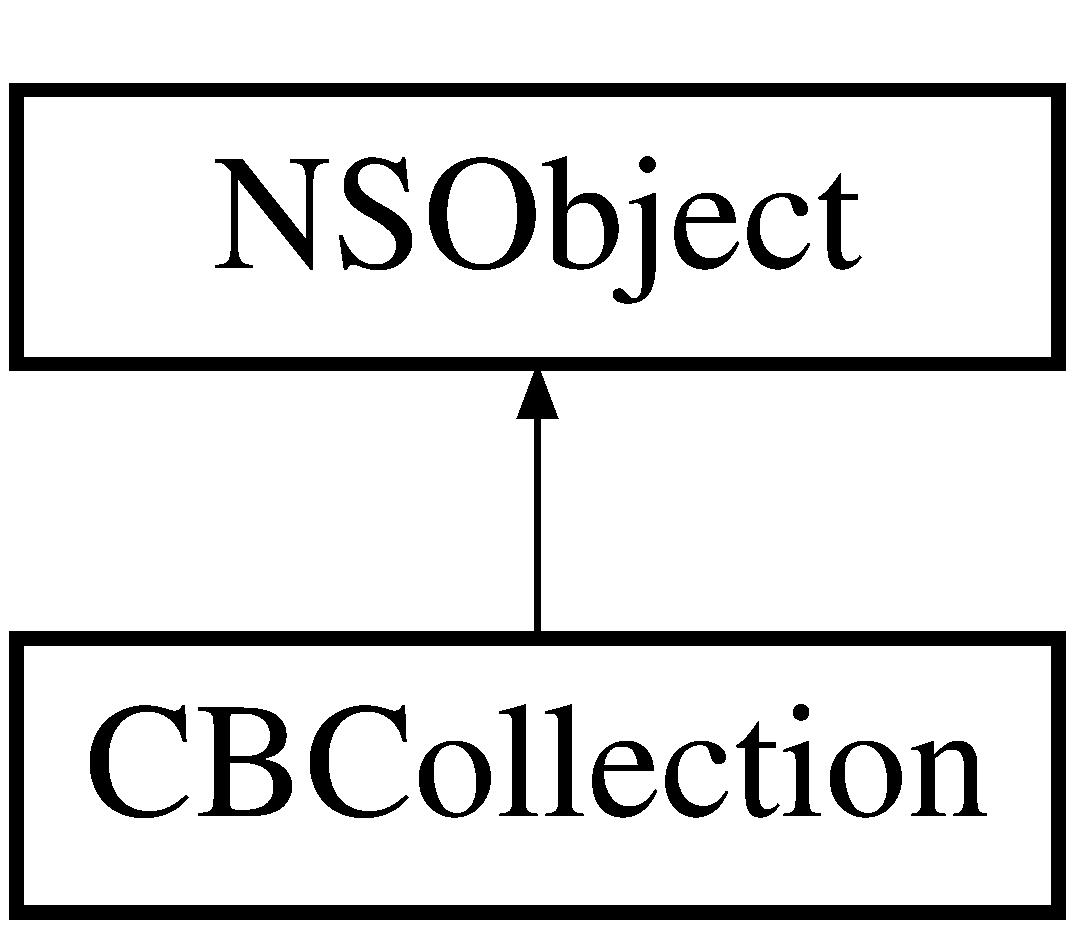
\includegraphics[height=2.000000cm]{interface_c_b_collection}
\end{center}
\end{figure}
\subsection*{Instance Methods}
\begin{DoxyCompactItemize}
\item 
(id) -\/ \hyperlink{interface_c_b_collection_ad232890eefe5c505991479ac6f018f9a}{init\+With\+Collection\+I\+D\+:}
\item 
(void) -\/ \hyperlink{interface_c_b_collection_aebbdb37306fcfa13bcdc915c96c37297}{fetch\+With\+Success\+Callback\+:with\+Error\+Callback\+:}
\item 
(void) -\/ \hyperlink{interface_c_b_collection_ad0e9afe7d01f2bf95510b1e462d31f2d}{fetch\+With\+Query\+:with\+Success\+Callback\+:with\+Error\+Callback\+:}
\item 
(void) -\/ \hyperlink{interface_c_b_collection_a72a5135772c9829d253fb614887158b4}{create\+With\+Data\+:with\+Success\+Callback\+:with\+Error\+Callback\+:}
\item 
(void) -\/ \hyperlink{interface_c_b_collection_af556b08ec3e81638b50b0bc8e06a9938}{update\+With\+Query\+:with\+Changes\+:with\+Success\+Callback\+:with\+Error\+Callback\+:}
\item 
(void) -\/ \hyperlink{interface_c_b_collection_a020a60192df9f85305aea894a19ac9ec}{remove\+With\+Query\+:with\+Success\+Callback\+:with\+Error\+Callback\+:}
\end{DoxyCompactItemize}
\subsection*{Class Methods}
\begin{DoxyCompactItemize}
\item 
(\hyperlink{interface_c_b_collection}{C\+B\+Collection} $\ast$) + \hyperlink{interface_c_b_collection_ad0d5e667992df0fbeedc094edd29375b}{collection\+With\+I\+D\+:}
\end{DoxyCompactItemize}
\subsection*{Properties}
\begin{DoxyCompactItemize}
\item 
N\+S\+String $\ast$ \hyperlink{interface_c_b_collection_a526d5990ac9db1922300bc55bc764fc1}{collection\+I\+D}
\end{DoxyCompactItemize}


\subsection{Detailed Description}
Class for dealing with \hyperlink{interface_clear_blade}{Clear\+Blade} Platform Collections. 

\subsection{Method Documentation}
\hypertarget{interface_c_b_collection_ad0d5e667992df0fbeedc094edd29375b}{\index{C\+B\+Collection@{C\+B\+Collection}!collection\+With\+I\+D\+:@{collection\+With\+I\+D\+:}}
\index{collection\+With\+I\+D\+:@{collection\+With\+I\+D\+:}!CBCollection@{C\+B\+Collection}}
\subsubsection[{collection\+With\+I\+D\+:}]{\setlength{\rightskip}{0pt plus 5cm}+ ({\bf C\+B\+Collection} $\ast$) collection\+With\+I\+D\+: 
\begin{DoxyParamCaption}
\item[{(N\+S\+String $\ast$)}]{collection\+I\+D}
\end{DoxyParamCaption}
}}\label{interface_c_b_collection_ad0d5e667992df0fbeedc094edd29375b}
Initialize a new \hyperlink{interface_c_b_collection}{C\+B\+Collection} object 
\begin{DoxyParams}{Parameters}
{\em collection\+I\+D} & The string that will be used to identify the collection on the server \\
\hline
\end{DoxyParams}
\begin{DoxyReturn}{Returns}
a newly initialized object 
\end{DoxyReturn}
\hypertarget{interface_c_b_collection_a72a5135772c9829d253fb614887158b4}{\index{C\+B\+Collection@{C\+B\+Collection}!create\+With\+Data\+:with\+Success\+Callback\+:with\+Error\+Callback\+:@{create\+With\+Data\+:with\+Success\+Callback\+:with\+Error\+Callback\+:}}
\index{create\+With\+Data\+:with\+Success\+Callback\+:with\+Error\+Callback\+:@{create\+With\+Data\+:with\+Success\+Callback\+:with\+Error\+Callback\+:}!CBCollection@{C\+B\+Collection}}
\subsubsection[{create\+With\+Data\+:with\+Success\+Callback\+:with\+Error\+Callback\+:}]{\setlength{\rightskip}{0pt plus 5cm}-\/ (void) create\+With\+Data\+: 
\begin{DoxyParamCaption}
\item[{(N\+S\+Dictionary $\ast$)}]{data}
\item[{withSuccessCallback:(C\+B\+Item\+Success\+Callback)}]{success\+Callback}
\item[{withErrorCallback:(C\+B\+Item\+Error\+Callback)}]{failure\+Callback}
\end{DoxyParamCaption}
}}\label{interface_c_b_collection_a72a5135772c9829d253fb614887158b4}
Creates a new Item in the collection in the Platform. This creates a new item on the server. 
\begin{DoxyParams}{Parameters}
{\em data} & A Dictionary that contains the object that you want the item in the platform to represent \\
\hline
{\em success\+Callback} & Callback Block to handle successfully returned data \\
\hline
{\em failure\+Callback} & Callback Block to handle errors returned \\
\hline
\end{DoxyParams}
\hypertarget{interface_c_b_collection_ad0e9afe7d01f2bf95510b1e462d31f2d}{\index{C\+B\+Collection@{C\+B\+Collection}!fetch\+With\+Query\+:with\+Success\+Callback\+:with\+Error\+Callback\+:@{fetch\+With\+Query\+:with\+Success\+Callback\+:with\+Error\+Callback\+:}}
\index{fetch\+With\+Query\+:with\+Success\+Callback\+:with\+Error\+Callback\+:@{fetch\+With\+Query\+:with\+Success\+Callback\+:with\+Error\+Callback\+:}!CBCollection@{C\+B\+Collection}}
\subsubsection[{fetch\+With\+Query\+:with\+Success\+Callback\+:with\+Error\+Callback\+:}]{\setlength{\rightskip}{0pt plus 5cm}-\/ (void) fetch\+With\+Query\+: 
\begin{DoxyParamCaption}
\item[{({\bf C\+B\+Query}$\ast$)}]{query}
\item[{withSuccessCallback:(C\+B\+Query\+Success\+Callback)}]{success\+Callback}
\item[{withErrorCallback:(C\+B\+Query\+Error\+Callback)}]{failure\+Callback}
\end{DoxyParamCaption}
}}\label{interface_c_b_collection_ad0e9afe7d01f2bf95510b1e462d31f2d}
Fetches all data from the collection that matches a particular query 
\begin{DoxyParams}{Parameters}
{\em query} & A \hyperlink{interface_c_b_query}{C\+B\+Query} object that defines what you want returned from the Platform \\
\hline
{\em success\+Callback} & Callback Block to handle successfully returned data \\
\hline
{\em failure\+Callback} & Callback Block to handle errors returned \\
\hline
\end{DoxyParams}
\hypertarget{interface_c_b_collection_aebbdb37306fcfa13bcdc915c96c37297}{\index{C\+B\+Collection@{C\+B\+Collection}!fetch\+With\+Success\+Callback\+:with\+Error\+Callback\+:@{fetch\+With\+Success\+Callback\+:with\+Error\+Callback\+:}}
\index{fetch\+With\+Success\+Callback\+:with\+Error\+Callback\+:@{fetch\+With\+Success\+Callback\+:with\+Error\+Callback\+:}!CBCollection@{C\+B\+Collection}}
\subsubsection[{fetch\+With\+Success\+Callback\+:with\+Error\+Callback\+:}]{\setlength{\rightskip}{0pt plus 5cm}-\/ (void) fetch\+With\+Success\+Callback\+: 
\begin{DoxyParamCaption}
\item[{(C\+B\+Query\+Success\+Callback)}]{success\+Callback}
\item[{withErrorCallback:(C\+B\+Query\+Error\+Callback)}]{failure\+Callback}
\end{DoxyParamCaption}
}}\label{interface_c_b_collection_aebbdb37306fcfa13bcdc915c96c37297}
Fetches the entire collection from the Platform. The returned data will be returned to the block you provide 
\begin{DoxyParams}{Parameters}
{\em success\+Callback} & Callback Block to handle successfully returned data \\
\hline
{\em failure\+Callback} & Callback Block to handle errors returned \\
\hline
\end{DoxyParams}
\hypertarget{interface_c_b_collection_ad232890eefe5c505991479ac6f018f9a}{\index{C\+B\+Collection@{C\+B\+Collection}!init\+With\+Collection\+I\+D\+:@{init\+With\+Collection\+I\+D\+:}}
\index{init\+With\+Collection\+I\+D\+:@{init\+With\+Collection\+I\+D\+:}!CBCollection@{C\+B\+Collection}}
\subsubsection[{init\+With\+Collection\+I\+D\+:}]{\setlength{\rightskip}{0pt plus 5cm}-\/ (id) init\+With\+Collection\+I\+D\+: 
\begin{DoxyParamCaption}
\item[{(N\+S\+String $\ast$)}]{col\+I\+D}
\end{DoxyParamCaption}
}}\label{interface_c_b_collection_ad232890eefe5c505991479ac6f018f9a}
Initialize a new \hyperlink{interface_c_b_collection}{C\+B\+Collection} object 
\begin{DoxyParams}{Parameters}
{\em col\+I\+D} & The string that will be used to identify the collection on the server \\
\hline
\end{DoxyParams}
\begin{DoxyReturn}{Returns}
a newly initialized object 
\end{DoxyReturn}
\hypertarget{interface_c_b_collection_a020a60192df9f85305aea894a19ac9ec}{\index{C\+B\+Collection@{C\+B\+Collection}!remove\+With\+Query\+:with\+Success\+Callback\+:with\+Error\+Callback\+:@{remove\+With\+Query\+:with\+Success\+Callback\+:with\+Error\+Callback\+:}}
\index{remove\+With\+Query\+:with\+Success\+Callback\+:with\+Error\+Callback\+:@{remove\+With\+Query\+:with\+Success\+Callback\+:with\+Error\+Callback\+:}!CBCollection@{C\+B\+Collection}}
\subsubsection[{remove\+With\+Query\+:with\+Success\+Callback\+:with\+Error\+Callback\+:}]{\setlength{\rightskip}{0pt plus 5cm}-\/ (void) remove\+With\+Query\+: 
\begin{DoxyParamCaption}
\item[{({\bf C\+B\+Query} $\ast$)}]{query}
\item[{withSuccessCallback:(C\+B\+Query\+Success\+Callback)}]{success\+Callback}
\item[{withErrorCallback:(C\+B\+Query\+Error\+Callback)}]{failure\+Callback}
\end{DoxyParamCaption}
}}\label{interface_c_b_collection_a020a60192df9f85305aea894a19ac9ec}
Removes an item or a set of items on the Platform that match the given query. 
\begin{DoxyParams}{Parameters}
{\em query} & A \hyperlink{interface_c_b_query}{C\+B\+Query} object that defines what you want removed from the Platform \\
\hline
{\em success\+Callback} & Callback Block to handle successfully returned data \\
\hline
{\em failure\+Callback} & Callback Block to handle errors returned \\
\hline
\end{DoxyParams}
\hypertarget{interface_c_b_collection_af556b08ec3e81638b50b0bc8e06a9938}{\index{C\+B\+Collection@{C\+B\+Collection}!update\+With\+Query\+:with\+Changes\+:with\+Success\+Callback\+:with\+Error\+Callback\+:@{update\+With\+Query\+:with\+Changes\+:with\+Success\+Callback\+:with\+Error\+Callback\+:}}
\index{update\+With\+Query\+:with\+Changes\+:with\+Success\+Callback\+:with\+Error\+Callback\+:@{update\+With\+Query\+:with\+Changes\+:with\+Success\+Callback\+:with\+Error\+Callback\+:}!CBCollection@{C\+B\+Collection}}
\subsubsection[{update\+With\+Query\+:with\+Changes\+:with\+Success\+Callback\+:with\+Error\+Callback\+:}]{\setlength{\rightskip}{0pt plus 5cm}-\/ (void) update\+With\+Query\+: 
\begin{DoxyParamCaption}
\item[{({\bf C\+B\+Query} $\ast$)}]{query}
\item[{withChanges:(N\+S\+Dictionary $\ast$)}]{changes}
\item[{withSuccessCallback:(C\+B\+Query\+Success\+Callback)}]{success\+Callback}
\item[{withErrorCallback:(C\+B\+Query\+Error\+Callback)}]{failure\+Callback}
\end{DoxyParamCaption}
}}\label{interface_c_b_collection_af556b08ec3e81638b50b0bc8e06a9938}
Updates an item or a set of items on the Platform that match the given query. 
\begin{DoxyParams}{Parameters}
{\em query} & A \hyperlink{interface_c_b_query}{C\+B\+Query} object that defines what you want updated on the Platform \\
\hline
{\em changes} & A Dictionary containing all of the changes that you want to make on items that match the query. \\
\hline
{\em success\+Callback} & Callback Block to handle successfully returned data \\
\hline
{\em failure\+Callback} & Callback Block to handle errors returned \\
\hline
\end{DoxyParams}


\subsection{Property Documentation}
\hypertarget{interface_c_b_collection_a526d5990ac9db1922300bc55bc764fc1}{\index{C\+B\+Collection@{C\+B\+Collection}!collection\+I\+D@{collection\+I\+D}}
\index{collection\+I\+D@{collection\+I\+D}!CBCollection@{C\+B\+Collection}}
\subsubsection[{collection\+I\+D}]{\setlength{\rightskip}{0pt plus 5cm}-\/ (N\+S\+String$\ast$) collection\+I\+D\hspace{0.3cm}{\ttfamily [read]}, {\ttfamily [write]}, {\ttfamily [nonatomic]}, {\ttfamily [strong]}}}\label{interface_c_b_collection_a526d5990ac9db1922300bc55bc764fc1}
The string that represents the collection I\+D. 

The documentation for this class was generated from the following files\+:\begin{DoxyCompactItemize}
\item 
C\+B\+Collection.\+h\item 
C\+B\+Collection.\+m\end{DoxyCompactItemize}

\hypertarget{interface_c_b_h_t_t_p_client}{\section{C\-B\-H\-T\-T\-P\-Client Class Reference}
\label{interface_c_b_h_t_t_p_client}\index{C\-B\-H\-T\-T\-P\-Client@{C\-B\-H\-T\-T\-P\-Client}}
}


{\ttfamily \#import $<$C\-B\-H\-T\-T\-P\-Client.\-h$>$}

Inheritance diagram for C\-B\-H\-T\-T\-P\-Client\-:\begin{figure}[H]
\begin{center}
\leavevmode
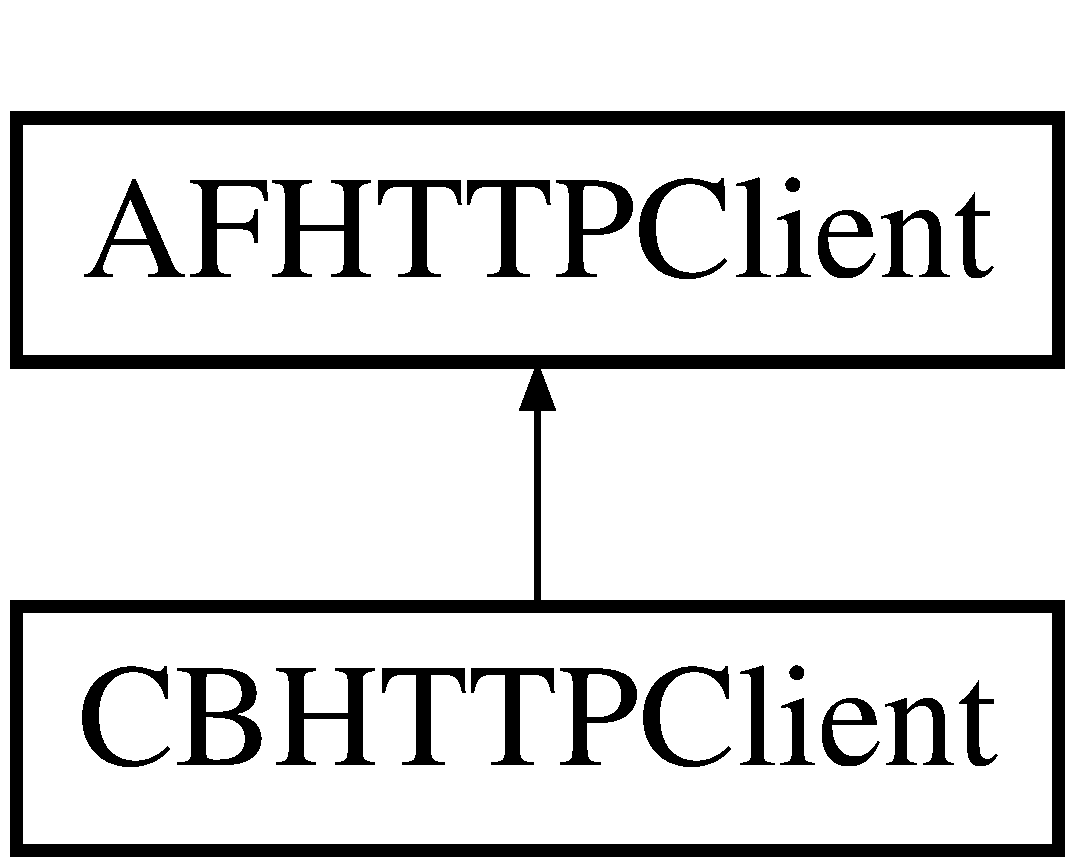
\includegraphics[height=2.000000cm]{interface_c_b_h_t_t_p_client}
\end{center}
\end{figure}
\subsection*{Instance Methods}
\begin{DoxyCompactItemize}
\item 
(void) -\/ \hyperlink{interface_c_b_h_t_t_p_client_ad5a36148d93216e8f41e81b4f0000d66}{set\-Url\-:}
\item 
(void) -\/ \hyperlink{interface_c_b_h_t_t_p_client_affe94c0f2e4358e5d8717f5af3cbb3e5}{set\-App\-Key\-:\-App\-Secret\-:}
\end{DoxyCompactItemize}
\subsection*{Properties}
\begin{DoxyCompactItemize}
\item 
N\-S\-U\-R\-L $\ast$ \hyperlink{interface_c_b_h_t_t_p_client_a9052e80b6482a3e1242f061b5f412df6}{base\-U\-R\-L}
\end{DoxyCompactItemize}


\subsection{Detailed Description}
Class used for making R\-E\-S\-T calls to the platform. This is a subclass of A\-F\-H\-T\-T\-P\-Client 

\subsection{Method Documentation}
\hypertarget{interface_c_b_h_t_t_p_client_affe94c0f2e4358e5d8717f5af3cbb3e5}{\index{C\-B\-H\-T\-T\-P\-Client@{C\-B\-H\-T\-T\-P\-Client}!set\-App\-Key\-:\-App\-Secret\-:@{set\-App\-Key\-:\-App\-Secret\-:}}
\index{set\-App\-Key\-:\-App\-Secret\-:@{set\-App\-Key\-:\-App\-Secret\-:}!CBHTTPClient@{C\-B\-H\-T\-T\-P\-Client}}
\subsubsection[{set\-App\-Key\-:\-App\-Secret\-:}]{\setlength{\rightskip}{0pt plus 5cm}-\/ (void) set\-App\-Key\-: 
\begin{DoxyParamCaption}
\item[{(N\-S\-String $\ast$)}]{key}
\item[{AppSecret:(N\-S\-String $\ast$)}]{secret}
\end{DoxyParamCaption}
}}\label{interface_c_b_h_t_t_p_client_affe94c0f2e4358e5d8717f5af3cbb3e5}
Sets that App\-Key and App\-Secret that get attached to the request headers for all requests to the platform 
\begin{DoxyParams}{Parameters}
{\em key} & The app key that is used to identify the app being used \\
\hline
{\em secret} & The app secret that is used to authenticate the app being used \\
\hline
\end{DoxyParams}
\hypertarget{interface_c_b_h_t_t_p_client_ad5a36148d93216e8f41e81b4f0000d66}{\index{C\-B\-H\-T\-T\-P\-Client@{C\-B\-H\-T\-T\-P\-Client}!set\-Url\-:@{set\-Url\-:}}
\index{set\-Url\-:@{set\-Url\-:}!CBHTTPClient@{C\-B\-H\-T\-T\-P\-Client}}
\subsubsection[{set\-Url\-:}]{\setlength{\rightskip}{0pt plus 5cm}-\/ (void) set\-Url\-: 
\begin{DoxyParamCaption}
\item[{(N\-S\-String $\ast$)}]{U\-R\-L}
\end{DoxyParamCaption}
}}\label{interface_c_b_h_t_t_p_client_ad5a36148d93216e8f41e81b4f0000d66}
Sets the base\-Url property that will be used by the client to communicate with the platform 
\begin{DoxyParams}{Parameters}
{\em U\-R\-L} & Tht N\-S\-U\-R\-L that is set as the base\-U\-R\-L \\
\hline
\end{DoxyParams}


\subsection{Property Documentation}
\hypertarget{interface_c_b_h_t_t_p_client_a9052e80b6482a3e1242f061b5f412df6}{\index{C\-B\-H\-T\-T\-P\-Client@{C\-B\-H\-T\-T\-P\-Client}!base\-U\-R\-L@{base\-U\-R\-L}}
\index{base\-U\-R\-L@{base\-U\-R\-L}!CBHTTPClient@{C\-B\-H\-T\-T\-P\-Client}}
\subsubsection[{base\-U\-R\-L}]{\setlength{\rightskip}{0pt plus 5cm}-\/ (N\-S\-U\-R\-L$\ast$) base\-U\-R\-L\hspace{0.3cm}{\ttfamily [read]}, {\ttfamily [write]}, {\ttfamily [nonatomic]}, {\ttfamily [strong]}}}\label{interface_c_b_h_t_t_p_client_a9052e80b6482a3e1242f061b5f412df6}
N\-S\-U\-R\-L that holds the url that the Client will use 

The documentation for this class was generated from the following files\-:\begin{DoxyCompactItemize}
\item 
C\-B\-H\-T\-T\-P\-Client.\-h\item 
C\-B\-H\-T\-T\-P\-Client.\-m\end{DoxyCompactItemize}

\hypertarget{interface_c_b_item}{\section{C\+B\+Item Class Reference}
\label{interface_c_b_item}\index{C\+B\+Item@{C\+B\+Item}}
}


{\ttfamily \#import $<$C\+B\+Item.\+h$>$}

Inheritance diagram for C\+B\+Item\+:\begin{figure}[H]
\begin{center}
\leavevmode
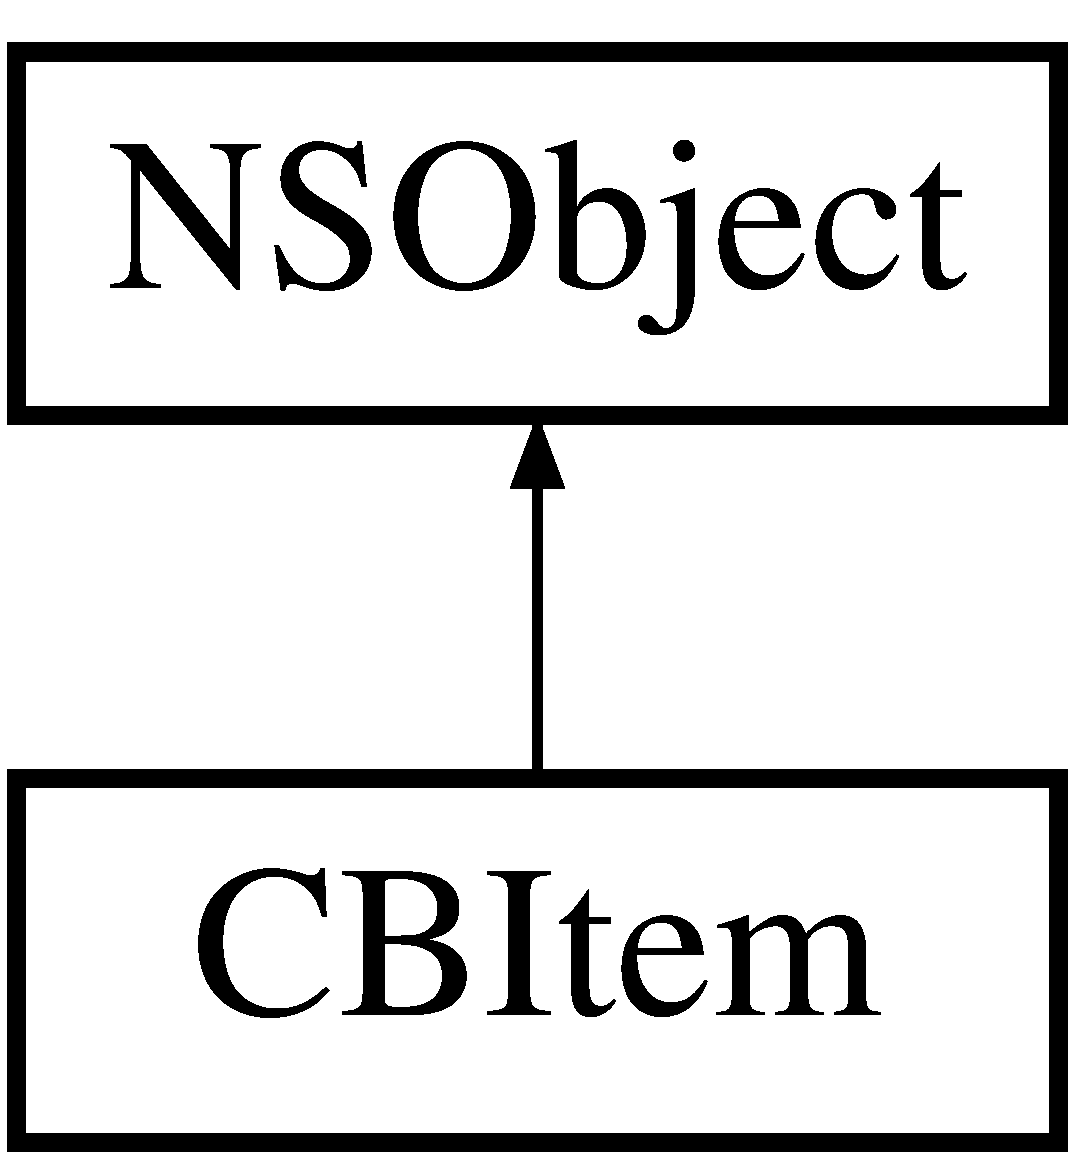
\includegraphics[height=2.000000cm]{interface_c_b_item}
\end{center}
\end{figure}
\subsection*{Instance Methods}
\begin{DoxyCompactItemize}
\item 
(instancetype) -\/ \hyperlink{interface_c_b_item_ace72b56932f3aa3b636800abdb50daa0}{init\+With\+Data\+:with\+Collection\+I\+D\+:}
\item 
(void) -\/ \hyperlink{interface_c_b_item_a35bde628ed02786ebcd145d74bea5ead}{save\+With\+Success\+Callback\+:with\+Error\+Callback\+:}
\item 
(void) -\/ \hyperlink{interface_c_b_item_acb4af198992cddea658fb099bbd81583}{refresh\+With\+Success\+Callback\+:with\+Error\+Callback\+:}
\item 
(void) -\/ \hyperlink{interface_c_b_item_acc375a79b97c2fcfaeda1c2737de51c0}{remove\+With\+Success\+Callback\+:with\+Error\+Callback\+:}
\item 
(id) -\/ \hyperlink{interface_c_b_item_aeb280c9120217ef525b1c47adb5db344}{object\+For\+Key\+:}
\item 
\hypertarget{interface_c_b_item_a850d0c9f26e8cd83ddec83458bc57df8}{(void) -\/ {\bfseries set\+Object\+:for\+Key\+:}}\label{interface_c_b_item_a850d0c9f26e8cd83ddec83458bc57df8}

\item 
(bool) -\/ \hyperlink{interface_c_b_item_ab47361f0044a8fd1893823b6ec95c46f}{is\+Equal\+To\+C\+B\+Item\+:}
\end{DoxyCompactItemize}
\subsection*{Class Methods}
\begin{DoxyCompactItemize}
\item 
(instancetype) + \hyperlink{interface_c_b_item_a5f9b22377c54afcb79916eaa66108140}{item\+With\+Data\+:with\+Collection\+I\+D\+:}
\item 
\hypertarget{interface_c_b_item_ab370a3dfb1ce240b8c59b41436532e56}{(N\+S\+Mutable\+Array $\ast$) + {\bfseries array\+Of\+C\+B\+Items\+From\+Array\+Of\+Dictionaries\+:with\+Collection\+I\+D\+:}}\label{interface_c_b_item_ab370a3dfb1ce240b8c59b41436532e56}

\end{DoxyCompactItemize}
\subsection*{Properties}
\begin{DoxyCompactItemize}
\item 
N\+S\+Mutable\+Dictionary $\ast$ \hyperlink{interface_c_b_item_a056a3d35cb718cb306dc69915bec29e2}{data}
\item 
N\+S\+String $\ast$ \hyperlink{interface_c_b_item_a8d47dba1bcfeb0754b65d312a48a939a}{collection\+I\+D}
\item 
N\+S\+String $\ast$ \hyperlink{interface_c_b_item_adc7d0932fa46e75354e7dbe63d714165}{item\+I\+D}
\end{DoxyCompactItemize}


\subsection{Detailed Description}
Class that represents an individual item from the platform 

\subsection{Method Documentation}
\hypertarget{interface_c_b_item_ace72b56932f3aa3b636800abdb50daa0}{\index{C\+B\+Item@{C\+B\+Item}!init\+With\+Data\+:with\+Collection\+I\+D\+:@{init\+With\+Data\+:with\+Collection\+I\+D\+:}}
\index{init\+With\+Data\+:with\+Collection\+I\+D\+:@{init\+With\+Data\+:with\+Collection\+I\+D\+:}!C\+B\+Item@{C\+B\+Item}}
\subsubsection[{init\+With\+Data\+:with\+Collection\+I\+D\+:}]{\setlength{\rightskip}{0pt plus 5cm}-\/ (instancetype) init\+With\+Data\+: 
\begin{DoxyParamCaption}
\item[{(N\+S\+Dictionary $\ast$)}]{input\+Data}
\item[{withCollectionID:(N\+S\+String $\ast$)}]{col\+I\+D}
\end{DoxyParamCaption}
}}\label{interface_c_b_item_ace72b56932f3aa3b636800abdb50daa0}
Initializes the Item with data and sets the data and collection\+I\+D. 
\begin{DoxyParams}{Parameters}
{\em input\+Data} & A dictionary that holds data for the item \\
\hline
{\em col\+I\+D} & A string that holds the I\+D of the collection to which this item belongs \\
\hline
\end{DoxyParams}
\begin{DoxyReturn}{Returns}
the newly created \hyperlink{interface_c_b_item}{C\+B\+Item} 
\end{DoxyReturn}
\hypertarget{interface_c_b_item_ab47361f0044a8fd1893823b6ec95c46f}{\index{C\+B\+Item@{C\+B\+Item}!is\+Equal\+To\+C\+B\+Item\+:@{is\+Equal\+To\+C\+B\+Item\+:}}
\index{is\+Equal\+To\+C\+B\+Item\+:@{is\+Equal\+To\+C\+B\+Item\+:}!C\+B\+Item@{C\+B\+Item}}
\subsubsection[{is\+Equal\+To\+C\+B\+Item\+:}]{\setlength{\rightskip}{0pt plus 5cm}-\/ (bool) is\+Equal\+To\+C\+B\+Item\+: 
\begin{DoxyParamCaption}
\item[{({\bf C\+B\+Item} $\ast$)}]{item}
\end{DoxyParamCaption}
}}\label{interface_c_b_item_ab47361f0044a8fd1893823b6ec95c46f}
Checks if all keys on both this \hyperlink{interface_c_b_item}{C\+B\+Item} and the other item are equal. 
\begin{DoxyParams}{Parameters}
{\em item} & The item to check against. \\
\hline
\end{DoxyParams}
\begin{DoxyReturn}{Returns}
true if the other item has all the same keys and values as this item. 
\end{DoxyReturn}
\hypertarget{interface_c_b_item_a5f9b22377c54afcb79916eaa66108140}{\index{C\+B\+Item@{C\+B\+Item}!item\+With\+Data\+:with\+Collection\+I\+D\+:@{item\+With\+Data\+:with\+Collection\+I\+D\+:}}
\index{item\+With\+Data\+:with\+Collection\+I\+D\+:@{item\+With\+Data\+:with\+Collection\+I\+D\+:}!C\+B\+Item@{C\+B\+Item}}
\subsubsection[{item\+With\+Data\+:with\+Collection\+I\+D\+:}]{\setlength{\rightskip}{0pt plus 5cm}+ ({\bf C\+B\+Item} $\ast$) item\+With\+Data\+: 
\begin{DoxyParamCaption}
\item[{(N\+S\+Dictionary $\ast$)}]{input\+Data}
\item[{withCollectionID:(N\+S\+String $\ast$)}]{collection\+I\+D}
\end{DoxyParamCaption}
}}\label{interface_c_b_item_a5f9b22377c54afcb79916eaa66108140}
Creates an Item with data belonging to the collection with collection\+I\+D 
\begin{DoxyParams}{Parameters}
{\em input\+Data} & A dictionary that holds data for the item \\
\hline
{\em collection\+I\+D} & The I\+D of the collection this item will belong to \\
\hline
\end{DoxyParams}
\begin{DoxyReturn}{Returns}
The newly created \hyperlink{interface_c_b_item}{C\+B\+Item} 
\end{DoxyReturn}
\hypertarget{interface_c_b_item_aeb280c9120217ef525b1c47adb5db344}{\index{C\+B\+Item@{C\+B\+Item}!object\+For\+Key\+:@{object\+For\+Key\+:}}
\index{object\+For\+Key\+:@{object\+For\+Key\+:}!C\+B\+Item@{C\+B\+Item}}
\subsubsection[{object\+For\+Key\+:}]{\setlength{\rightskip}{0pt plus 5cm}-\/ (id) object\+For\+Key\+: 
\begin{DoxyParamCaption}
\item[{(N\+S\+String $\ast$)}]{key}
\end{DoxyParamCaption}
}}\label{interface_c_b_item_aeb280c9120217ef525b1c47adb5db344}
Gets an item out of the data attribute that matches the given string 
\begin{DoxyParams}{Parameters}
{\em key} & String used to find a value in the dictionary \\
\hline
\end{DoxyParams}
\begin{DoxyReturn}{Returns}
The id that is referenced by the value for the given key 
\end{DoxyReturn}
\hypertarget{interface_c_b_item_acb4af198992cddea658fb099bbd81583}{\index{C\+B\+Item@{C\+B\+Item}!refresh\+With\+Success\+Callback\+:with\+Error\+Callback\+:@{refresh\+With\+Success\+Callback\+:with\+Error\+Callback\+:}}
\index{refresh\+With\+Success\+Callback\+:with\+Error\+Callback\+:@{refresh\+With\+Success\+Callback\+:with\+Error\+Callback\+:}!C\+B\+Item@{C\+B\+Item}}
\subsubsection[{refresh\+With\+Success\+Callback\+:with\+Error\+Callback\+:}]{\setlength{\rightskip}{0pt plus 5cm}-\/ (void) refresh\+With\+Success\+Callback\+: 
\begin{DoxyParamCaption}
\item[{(C\+B\+Item\+Success\+Callback)}]{success\+Callback}
\item[{withErrorCallback:(C\+B\+Item\+Error\+Callback)}]{error\+Callback}
\end{DoxyParamCaption}
}}\label{interface_c_b_item_acb4af198992cddea658fb099bbd81583}
Pulls down any changes that have been made on the server to the item since being instantiated. This updates the data attribute to reflect the current state of the Item on the server \hypertarget{interface_c_b_item_acc375a79b97c2fcfaeda1c2737de51c0}{\index{C\+B\+Item@{C\+B\+Item}!remove\+With\+Success\+Callback\+:with\+Error\+Callback\+:@{remove\+With\+Success\+Callback\+:with\+Error\+Callback\+:}}
\index{remove\+With\+Success\+Callback\+:with\+Error\+Callback\+:@{remove\+With\+Success\+Callback\+:with\+Error\+Callback\+:}!C\+B\+Item@{C\+B\+Item}}
\subsubsection[{remove\+With\+Success\+Callback\+:with\+Error\+Callback\+:}]{\setlength{\rightskip}{0pt plus 5cm}-\/ (void) remove\+With\+Success\+Callback\+: 
\begin{DoxyParamCaption}
\item[{(C\+B\+Item\+Success\+Callback)}]{success\+Callback}
\item[{withErrorCallback:(C\+B\+Item\+Error\+Callback)}]{error\+Callback}
\end{DoxyParamCaption}
}}\label{interface_c_b_item_acc375a79b97c2fcfaeda1c2737de51c0}
Deletes the Item on the server This cannot be undone. \hypertarget{interface_c_b_item_a35bde628ed02786ebcd145d74bea5ead}{\index{C\+B\+Item@{C\+B\+Item}!save\+With\+Success\+Callback\+:with\+Error\+Callback\+:@{save\+With\+Success\+Callback\+:with\+Error\+Callback\+:}}
\index{save\+With\+Success\+Callback\+:with\+Error\+Callback\+:@{save\+With\+Success\+Callback\+:with\+Error\+Callback\+:}!C\+B\+Item@{C\+B\+Item}}
\subsubsection[{save\+With\+Success\+Callback\+:with\+Error\+Callback\+:}]{\setlength{\rightskip}{0pt plus 5cm}-\/ (void) save\+With\+Success\+Callback\+: 
\begin{DoxyParamCaption}
\item[{(C\+B\+Item\+Success\+Callback)}]{success\+Callback}
\item[{withErrorCallback:(C\+B\+Item\+Error\+Callback)}]{error\+Callback}
\end{DoxyParamCaption}
}}\label{interface_c_b_item_a35bde628ed02786ebcd145d74bea5ead}
Saves any changes that have been made to the data property to the Platform This will update the server 

\subsection{Property Documentation}
\hypertarget{interface_c_b_item_a8d47dba1bcfeb0754b65d312a48a939a}{\index{C\+B\+Item@{C\+B\+Item}!collection\+I\+D@{collection\+I\+D}}
\index{collection\+I\+D@{collection\+I\+D}!C\+B\+Item@{C\+B\+Item}}
\subsubsection[{collection\+I\+D}]{\setlength{\rightskip}{0pt plus 5cm}-\/ (N\+S\+String$\ast$) collection\+I\+D\hspace{0.3cm}{\ttfamily [read]}, {\ttfamily [write]}, {\ttfamily [nonatomic]}, {\ttfamily [strong]}}}\label{interface_c_b_item_a8d47dba1bcfeb0754b65d312a48a939a}
A string holding the I\+D of the collection to which this item belongs \hypertarget{interface_c_b_item_a056a3d35cb718cb306dc69915bec29e2}{\index{C\+B\+Item@{C\+B\+Item}!data@{data}}
\index{data@{data}!C\+B\+Item@{C\+B\+Item}}
\subsubsection[{data}]{\setlength{\rightskip}{0pt plus 5cm}-\/ (N\+S\+Mutable\+Dictionary $\ast$) data\hspace{0.3cm}{\ttfamily [read]}, {\ttfamily [write]}, {\ttfamily [nonatomic]}, {\ttfamily [strong]}}}\label{interface_c_b_item_a056a3d35cb718cb306dc69915bec29e2}
A dictionary that holds the data that was stored in the platform. \hypertarget{interface_c_b_item_adc7d0932fa46e75354e7dbe63d714165}{\index{C\+B\+Item@{C\+B\+Item}!item\+I\+D@{item\+I\+D}}
\index{item\+I\+D@{item\+I\+D}!C\+B\+Item@{C\+B\+Item}}
\subsubsection[{item\+I\+D}]{\setlength{\rightskip}{0pt plus 5cm}-\/ (N\+S\+String $\ast$) item\+I\+D\hspace{0.3cm}{\ttfamily [read]}, {\ttfamily [write]}, {\ttfamily [nonatomic]}, {\ttfamily [strong]}}}\label{interface_c_b_item_adc7d0932fa46e75354e7dbe63d714165}
A string holding the I\+D of the item 

The documentation for this class was generated from the following files\+:\begin{DoxyCompactItemize}
\item 
Clear\+Blade\+A\+P\+I/C\+B\+Item.\+h\item 
Clear\+Blade\+A\+P\+I/C\+B\+Item.\+m\end{DoxyCompactItemize}

\hypertarget{interface_c_b_query}{\section{C\+B\+Query Class Reference}
\label{interface_c_b_query}\index{C\+B\+Query@{C\+B\+Query}}
}


{\ttfamily \#import $<$C\+B\+Query.\+h$>$}

Inheritance diagram for C\+B\+Query\+:\begin{figure}[H]
\begin{center}
\leavevmode
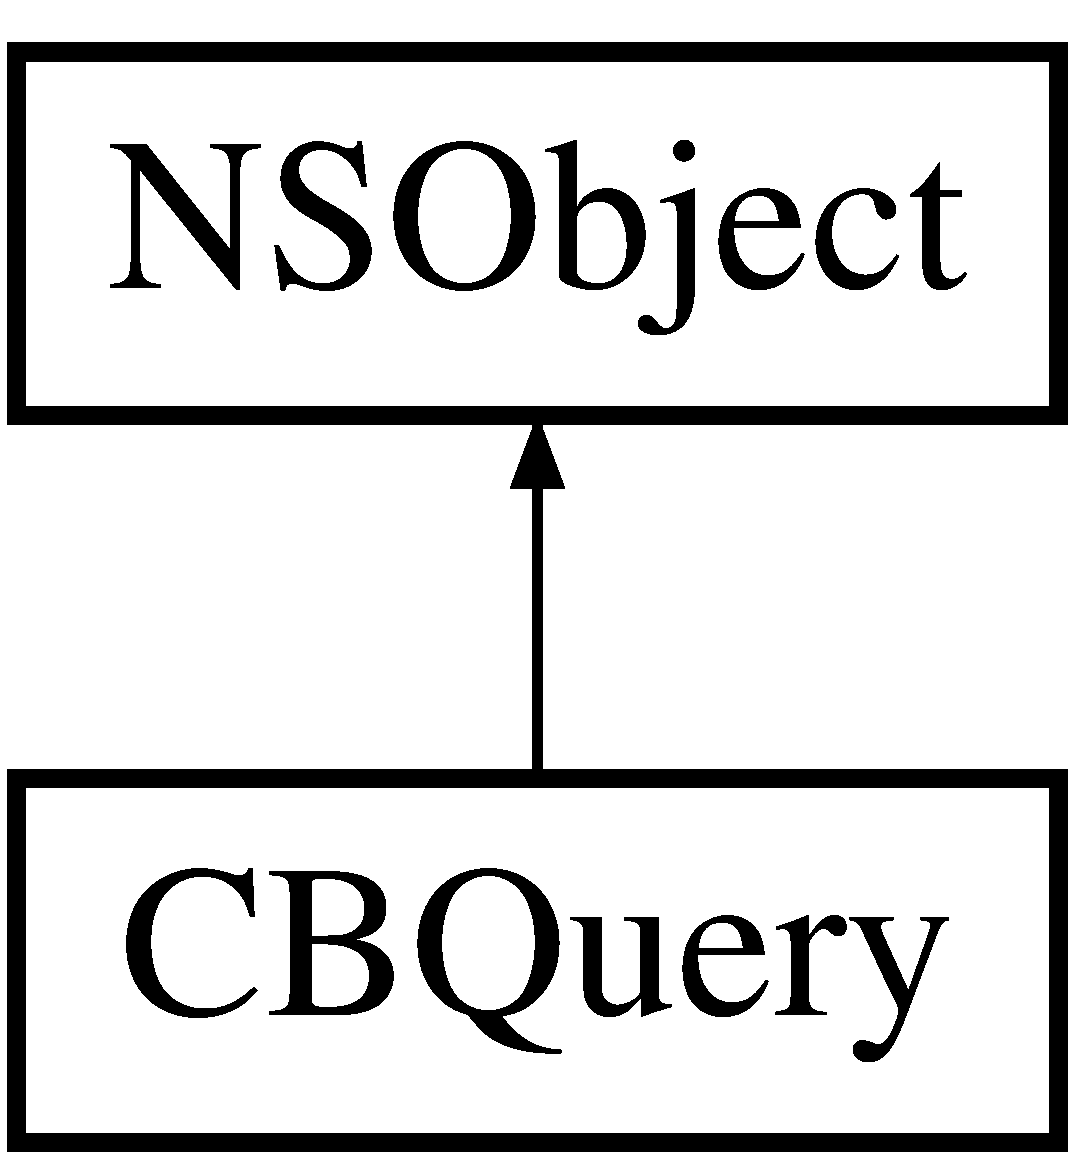
\includegraphics[height=2.000000cm]{interface_c_b_query}
\end{center}
\end{figure}
\subsection*{Instance Methods}
\begin{DoxyCompactItemize}
\item 
(\hyperlink{interface_c_b_query}{C\+B\+Query} $\ast$) -\/ \hyperlink{interface_c_b_query_a945b8a169282151a97e6a0fd694cbb33}{init\+With\+Collection\+I\+D\+:}
\item 
(void) -\/ \hyperlink{interface_c_b_query_aa6df57d4b22629273cb22d39157ab234}{set\+Collection\+I\+D\+:}
\item 
(void) -\/ \hyperlink{interface_c_b_query_a2ff55cfdc8420ce06c3bfe334691a7cd}{fetch\+With\+Success\+Callback\+:with\+Error\+Callback\+:}
\item 
(void) -\/ \hyperlink{interface_c_b_query_aca3f69cedd6770da3fac14535b050d6c}{update\+With\+Changes\+:with\+Success\+Callback\+:with\+Error\+Callback\+:}
\item 
(void) -\/ \hyperlink{interface_c_b_query_a7c2529e9ef2e4c3630b01d8bff1ea25b}{insert\+Item\+:into\+Collection\+With\+I\+D\+:with\+Success\+Callback\+:with\+Error\+Callback\+:}
\item 
(void) -\/ \hyperlink{interface_c_b_query_acecf2b37deaf04803066830664b81ad1}{remove\+With\+Success\+Callback\+:with\+Error\+Callback\+:}
\item 
(\hyperlink{interface_c_b_query}{C\+B\+Query} $\ast$) -\/ \hyperlink{interface_c_b_query_a3ff649bb71392f2f21e210f07f0ef761}{equal\+To\+:for\+:}
\item 
(\hyperlink{interface_c_b_query}{C\+B\+Query} $\ast$) -\/ \hyperlink{interface_c_b_query_af7920062116379d99531b3443a8c3aa3}{not\+Equal\+To\+:for\+:}
\item 
(\hyperlink{interface_c_b_query}{C\+B\+Query} $\ast$) -\/ \hyperlink{interface_c_b_query_a26d58f8c51997aea862c26cc291d743e}{greater\+Than\+:for\+:}
\item 
(\hyperlink{interface_c_b_query}{C\+B\+Query} $\ast$) -\/ \hyperlink{interface_c_b_query_a29af545dcdf721cae1534c219a991021}{less\+Than\+:for\+:}
\item 
(\hyperlink{interface_c_b_query}{C\+B\+Query} $\ast$) -\/ \hyperlink{interface_c_b_query_a52b23279069fa19429ed6473ecf0eb73}{greater\+Than\+Equal\+To\+:for\+:}
\item 
(\hyperlink{interface_c_b_query}{C\+B\+Query} $\ast$) -\/ \hyperlink{interface_c_b_query_ac8007f263dbc069970ee76c90666b043}{less\+Than\+Equal\+To\+:for\+:}
\item 
(\hyperlink{interface_c_b_query}{C\+B\+Query} $\ast$) -\/ \hyperlink{interface_c_b_query_a5d7977f390caeb0eccb620ddf6e24c2f}{set\+Page\+Size\+:}
\item 
(\hyperlink{interface_c_b_query}{C\+B\+Query} $\ast$) -\/ \hyperlink{interface_c_b_query_a04a966e136634595b92597e8437ff176}{set\+Page\+Num\+:}
\item 
(\hyperlink{interface_c_b_query}{C\+B\+Query} $\ast$) -\/ \hyperlink{interface_c_b_query_abcb133d3ea6c27ccd85fc9d1278f7f41}{add\+Query\+As\+Or\+Clause\+Using\+Query\+:}
\end{DoxyCompactItemize}
\subsection*{Class Methods}
\begin{DoxyCompactItemize}
\item 
(\hyperlink{interface_c_b_query}{C\+B\+Query} $\ast$) + \hyperlink{interface_c_b_query_a616541706465f78433a3b2488760df4f}{query\+With\+Collection\+I\+D\+:}
\end{DoxyCompactItemize}
\subsection*{Properties}
\begin{DoxyCompactItemize}
\item 
N\+S\+String $\ast$ \hyperlink{interface_c_b_query_ad7e594dc30699c9dbae407e55b588b00}{collection\+I\+D}
\item 
\hyperlink{interface_c_b_user}{C\+B\+User} $\ast$ \hyperlink{interface_c_b_query_af5679b48acc1313cab6dd83e2777b440}{user}
\end{DoxyCompactItemize}


\subsection{Detailed Description}
Class representing a query that can be used in operations on Platform 

\subsection{Method Documentation}
\hypertarget{interface_c_b_query_abcb133d3ea6c27ccd85fc9d1278f7f41}{\index{C\+B\+Query@{C\+B\+Query}!add\+Query\+As\+Or\+Clause\+Using\+Query\+:@{add\+Query\+As\+Or\+Clause\+Using\+Query\+:}}
\index{add\+Query\+As\+Or\+Clause\+Using\+Query\+:@{add\+Query\+As\+Or\+Clause\+Using\+Query\+:}!CBQuery@{C\+B\+Query}}
\subsubsection[{add\+Query\+As\+Or\+Clause\+Using\+Query\+:}]{\setlength{\rightskip}{0pt plus 5cm}-\/ ({\bf C\+B\+Query} $\ast$) add\+Query\+As\+Or\+Clause\+Using\+Query\+: 
\begin{DoxyParamCaption}
\item[{({\bf C\+B\+Query} $\ast$)}]{or\+Query}
\end{DoxyParamCaption}
}}\label{interface_c_b_query_abcb133d3ea6c27ccd85fc9d1278f7f41}
Adds another \hyperlink{interface_c_b_query}{C\+B\+Query} as an O\+R clause. This allows you to create two separate \hyperlink{interface_c_b_query}{C\+B\+Query} objects to then O\+R together. This operation happens in place so the caller's underlying query is changed but the Query used as the argument is not. 
\begin{DoxyParams}{Parameters}
{\em or\+Query} & A \hyperlink{interface_c_b_query}{C\+B\+Query} to be O\+R'd to the calling \hyperlink{interface_c_b_query}{C\+B\+Query}.\\
\hline
\end{DoxyParams}
Example\+: \hyperlink{interface_c_b_query}{C\+B\+Query} $\ast$first\+Query = \mbox{[}\hyperlink{interface_c_b_query}{C\+B\+Query} query\+With\+Collection\+I\+D\+:"f28faaa10a8ca5a5f2f5acd297cc01\char`\"{}\mbox{]}
\mbox{[}first\+Query equal\+To\+:@\char`\"{}value1\char`\"{} for\+:@\char`\"{}key1\char`\"{}\mbox{]}
\mbox{[}first\+Query equal\+To\+:@\char`\"{}value2\char`\"{} for\+:@\char`\"{}key2\char`\"{}\mbox{]}
\+C\+B\+Query $\ast$second\+Query = \mbox{[}\+C\+B\+Query query\+With\+Collection\+I\+D\+:@\char`\"{}f28faaa10a8ca5a5f2f5acd297cc01\char`\"{}\mbox{]}
\mbox{[}second\+Query equal\+To@\char`\"{}value3\char`\"{} for\+:@\char`\"{}key3"\mbox{]} \hyperlink{interface_c_b_query}{C\+B\+Query} $\ast$third\+Query = \mbox{[}first\+Query add\+Query\+As\+Or\+Clause\+Using\+Query\+:second\+Query\mbox{]}

In the example, third\+Query would be equivalent to this S\+Q\+L\+: W\+H\+E\+R\+E \char`\"{}key1\char`\"{} = \char`\"{}value1\char`\"{} A\+N\+D \char`\"{}key2\char`\"{} = \char`\"{}value2\char`\"{} O\+R \char`\"{}key3\char`\"{} = \char`\"{}value3\char`\"{} \hypertarget{interface_c_b_query_a3ff649bb71392f2f21e210f07f0ef761}{\index{C\+B\+Query@{C\+B\+Query}!equal\+To\+:for\+:@{equal\+To\+:for\+:}}
\index{equal\+To\+:for\+:@{equal\+To\+:for\+:}!CBQuery@{C\+B\+Query}}
\subsubsection[{equal\+To\+:for\+:}]{\setlength{\rightskip}{0pt plus 5cm}-\/ ({\bf C\+B\+Query} $\ast$) equal\+To\+: 
\begin{DoxyParamCaption}
\item[{(id)}]{value}
\item[{for:(N\+S\+String $\ast$)}]{key}
\end{DoxyParamCaption}
}}\label{interface_c_b_query_a3ff649bb71392f2f21e210f07f0ef761}
Creates an equality clause and adds it to the query 
\begin{DoxyParams}{Parameters}
{\em value} & A string that gets set as the value for the given key \\
\hline
{\em key} & A string that is used as the key for the given value \\
\hline
\end{DoxyParams}
\begin{DoxyReturn}{Returns}
The query with the new clause added 
\end{DoxyReturn}
\hypertarget{interface_c_b_query_a2ff55cfdc8420ce06c3bfe334691a7cd}{\index{C\+B\+Query@{C\+B\+Query}!fetch\+With\+Success\+Callback\+:with\+Error\+Callback\+:@{fetch\+With\+Success\+Callback\+:with\+Error\+Callback\+:}}
\index{fetch\+With\+Success\+Callback\+:with\+Error\+Callback\+:@{fetch\+With\+Success\+Callback\+:with\+Error\+Callback\+:}!CBQuery@{C\+B\+Query}}
\subsubsection[{fetch\+With\+Success\+Callback\+:with\+Error\+Callback\+:}]{\setlength{\rightskip}{0pt plus 5cm}-\/ (void) fetch\+With\+Success\+Callback\+: 
\begin{DoxyParamCaption}
\item[{(C\+B\+Query\+Success\+Callback)}]{success\+Callback}
\item[{withErrorCallback:(C\+B\+Query\+Error\+Callback)}]{failure\+Callback}
\end{DoxyParamCaption}
}}\label{interface_c_b_query_a2ff55cfdc8420ce06c3bfe334691a7cd}
Fetches from a collection all of the items that match the query that is sent. 
\begin{DoxyParams}{Parameters}
{\em success\+Callback} & A callback block that handles the returned data \\
\hline
{\em failure\+Callback} & A callback block that handles errors returned \\
\hline
\end{DoxyParams}
\hypertarget{interface_c_b_query_a26d58f8c51997aea862c26cc291d743e}{\index{C\+B\+Query@{C\+B\+Query}!greater\+Than\+:for\+:@{greater\+Than\+:for\+:}}
\index{greater\+Than\+:for\+:@{greater\+Than\+:for\+:}!CBQuery@{C\+B\+Query}}
\subsubsection[{greater\+Than\+:for\+:}]{\setlength{\rightskip}{0pt plus 5cm}-\/ ({\bf C\+B\+Query} $\ast$) greater\+Than\+: 
\begin{DoxyParamCaption}
\item[{(N\+S\+Number $\ast$)}]{value}
\item[{for:(N\+S\+String $\ast$)}]{key}
\end{DoxyParamCaption}
}}\label{interface_c_b_query_a26d58f8c51997aea862c26cc291d743e}
Creates a greater than clause and adds it to the query 
\begin{DoxyParams}{Parameters}
{\em value} & A string that gets set as the value for the given key \\
\hline
{\em key} & A string that is used as the key for the given value \\
\hline
\end{DoxyParams}
\begin{DoxyReturn}{Returns}
The query with the new clause added 
\end{DoxyReturn}
\hypertarget{interface_c_b_query_a52b23279069fa19429ed6473ecf0eb73}{\index{C\+B\+Query@{C\+B\+Query}!greater\+Than\+Equal\+To\+:for\+:@{greater\+Than\+Equal\+To\+:for\+:}}
\index{greater\+Than\+Equal\+To\+:for\+:@{greater\+Than\+Equal\+To\+:for\+:}!CBQuery@{C\+B\+Query}}
\subsubsection[{greater\+Than\+Equal\+To\+:for\+:}]{\setlength{\rightskip}{0pt plus 5cm}-\/ ({\bf C\+B\+Query} $\ast$) greater\+Than\+Equal\+To\+: 
\begin{DoxyParamCaption}
\item[{(N\+S\+Number $\ast$)}]{value}
\item[{for:(N\+S\+String $\ast$)}]{key}
\end{DoxyParamCaption}
}}\label{interface_c_b_query_a52b23279069fa19429ed6473ecf0eb73}
Creates a greater than or equal to clause and adds it to the query 
\begin{DoxyParams}{Parameters}
{\em value} & A string that gets set as the value for the given key \\
\hline
{\em key} & A string that is used as the key for the given value \\
\hline
\end{DoxyParams}
\begin{DoxyReturn}{Returns}
The query with the new clause added 
\end{DoxyReturn}
\hypertarget{interface_c_b_query_a945b8a169282151a97e6a0fd694cbb33}{\index{C\+B\+Query@{C\+B\+Query}!init\+With\+Collection\+I\+D\+:@{init\+With\+Collection\+I\+D\+:}}
\index{init\+With\+Collection\+I\+D\+:@{init\+With\+Collection\+I\+D\+:}!CBQuery@{C\+B\+Query}}
\subsubsection[{init\+With\+Collection\+I\+D\+:}]{\setlength{\rightskip}{0pt plus 5cm}-\/ ({\bf C\+B\+Query} $\ast$) init\+With\+Collection\+I\+D\+: 
\begin{DoxyParamCaption}
\item[{(N\+S\+String $\ast$)}]{col\+I\+D}
\end{DoxyParamCaption}
}}\label{interface_c_b_query_a945b8a169282151a97e6a0fd694cbb33}
Initializes the query object and sets the collection\+I\+D 
\begin{DoxyParams}{Parameters}
{\em col\+I\+D} & A string that is set as collection\+I\+D \\
\hline
\end{DoxyParams}
\begin{DoxyReturn}{Returns}
the newly instantiated \hyperlink{interface_c_b_query}{C\+B\+Query} Object 
\end{DoxyReturn}
\hypertarget{interface_c_b_query_a7c2529e9ef2e4c3630b01d8bff1ea25b}{\index{C\+B\+Query@{C\+B\+Query}!insert\+Item\+:into\+Collection\+With\+I\+D\+:with\+Success\+Callback\+:with\+Error\+Callback\+:@{insert\+Item\+:into\+Collection\+With\+I\+D\+:with\+Success\+Callback\+:with\+Error\+Callback\+:}}
\index{insert\+Item\+:into\+Collection\+With\+I\+D\+:with\+Success\+Callback\+:with\+Error\+Callback\+:@{insert\+Item\+:into\+Collection\+With\+I\+D\+:with\+Success\+Callback\+:with\+Error\+Callback\+:}!CBQuery@{C\+B\+Query}}
\subsubsection[{insert\+Item\+:into\+Collection\+With\+I\+D\+:with\+Success\+Callback\+:with\+Error\+Callback\+:}]{\setlength{\rightskip}{0pt plus 5cm}-\/ (void) insert\+Item\+: 
\begin{DoxyParamCaption}
\item[{({\bf C\+B\+Item} $\ast$)}]{item}
\item[{intoCollectionWithID:(N\+S\+String $\ast$)}]{collection\+I\+D}
\item[{withSuccessCallback:(C\+B\+Operation\+Success\+Callback)}]{success\+Callback}
\item[{withErrorCallback:(C\+B\+Query\+Error\+Callback)}]{error\+Callback}
\end{DoxyParamCaption}
}}\label{interface_c_b_query_a7c2529e9ef2e4c3630b01d8bff1ea25b}
Inserts the object into the collection. Ignores any query parameters 
\begin{DoxyParams}{Parameters}
{\em item} & The item to be inserted into the collection \\
\hline
{\em collection\+I\+D} & The I\+D of the collection to insert the item into \\
\hline
{\em success\+Callback} & A callback block that handles the return data \\
\hline
{\em error\+Callback} & A callback block that handles the errors returned \\
\hline
\end{DoxyParams}
\hypertarget{interface_c_b_query_a29af545dcdf721cae1534c219a991021}{\index{C\+B\+Query@{C\+B\+Query}!less\+Than\+:for\+:@{less\+Than\+:for\+:}}
\index{less\+Than\+:for\+:@{less\+Than\+:for\+:}!CBQuery@{C\+B\+Query}}
\subsubsection[{less\+Than\+:for\+:}]{\setlength{\rightskip}{0pt plus 5cm}-\/ ({\bf C\+B\+Query} $\ast$) less\+Than\+: 
\begin{DoxyParamCaption}
\item[{(N\+S\+Number $\ast$)}]{value}
\item[{for:(N\+S\+String $\ast$)}]{key}
\end{DoxyParamCaption}
}}\label{interface_c_b_query_a29af545dcdf721cae1534c219a991021}
Creates a less than clause and adds it to the query 
\begin{DoxyParams}{Parameters}
{\em value} & A string that gets set as the value for the given key \\
\hline
{\em key} & A string that is used as the key for the given value \\
\hline
\end{DoxyParams}
\begin{DoxyReturn}{Returns}
The query with the new clause added 
\end{DoxyReturn}
\hypertarget{interface_c_b_query_ac8007f263dbc069970ee76c90666b043}{\index{C\+B\+Query@{C\+B\+Query}!less\+Than\+Equal\+To\+:for\+:@{less\+Than\+Equal\+To\+:for\+:}}
\index{less\+Than\+Equal\+To\+:for\+:@{less\+Than\+Equal\+To\+:for\+:}!CBQuery@{C\+B\+Query}}
\subsubsection[{less\+Than\+Equal\+To\+:for\+:}]{\setlength{\rightskip}{0pt plus 5cm}-\/ ({\bf C\+B\+Query} $\ast$) less\+Than\+Equal\+To\+: 
\begin{DoxyParamCaption}
\item[{(N\+S\+Number $\ast$)}]{value}
\item[{for:(N\+S\+String $\ast$)}]{key}
\end{DoxyParamCaption}
}}\label{interface_c_b_query_ac8007f263dbc069970ee76c90666b043}
Creates a less than or equal to clause and adds it to the query 
\begin{DoxyParams}{Parameters}
{\em value} & A string that gets set as the value for the given key \\
\hline
{\em key} & A string that is used as the key for the given value \\
\hline
\end{DoxyParams}
\begin{DoxyReturn}{Returns}
The query with the new clause added 
\end{DoxyReturn}
\hypertarget{interface_c_b_query_af7920062116379d99531b3443a8c3aa3}{\index{C\+B\+Query@{C\+B\+Query}!not\+Equal\+To\+:for\+:@{not\+Equal\+To\+:for\+:}}
\index{not\+Equal\+To\+:for\+:@{not\+Equal\+To\+:for\+:}!CBQuery@{C\+B\+Query}}
\subsubsection[{not\+Equal\+To\+:for\+:}]{\setlength{\rightskip}{0pt plus 5cm}-\/ ({\bf C\+B\+Query} $\ast$) not\+Equal\+To\+: 
\begin{DoxyParamCaption}
\item[{(id)}]{value}
\item[{for:(N\+S\+String $\ast$)}]{key}
\end{DoxyParamCaption}
}}\label{interface_c_b_query_af7920062116379d99531b3443a8c3aa3}
Creates an inequality clause and adds it to the query 
\begin{DoxyParams}{Parameters}
{\em value} & A string that gets set as the value for the given key \\
\hline
{\em key} & A string that is used as the key for the given value \\
\hline
\end{DoxyParams}
\begin{DoxyReturn}{Returns}
The query with the new clause added 
\end{DoxyReturn}
\hypertarget{interface_c_b_query_a616541706465f78433a3b2488760df4f}{\index{C\+B\+Query@{C\+B\+Query}!query\+With\+Collection\+I\+D\+:@{query\+With\+Collection\+I\+D\+:}}
\index{query\+With\+Collection\+I\+D\+:@{query\+With\+Collection\+I\+D\+:}!CBQuery@{C\+B\+Query}}
\subsubsection[{query\+With\+Collection\+I\+D\+:}]{\setlength{\rightskip}{0pt plus 5cm}+ ({\bf C\+B\+Query} $\ast$) query\+With\+Collection\+I\+D\+: 
\begin{DoxyParamCaption}
\item[{(N\+S\+String $\ast$)}]{collection\+I\+D}
\end{DoxyParamCaption}
}}\label{interface_c_b_query_a616541706465f78433a3b2488760df4f}
Creates a query object that will operate on the collection with the collection\+I\+D \hypertarget{interface_c_b_query_acecf2b37deaf04803066830664b81ad1}{\index{C\+B\+Query@{C\+B\+Query}!remove\+With\+Success\+Callback\+:with\+Error\+Callback\+:@{remove\+With\+Success\+Callback\+:with\+Error\+Callback\+:}}
\index{remove\+With\+Success\+Callback\+:with\+Error\+Callback\+:@{remove\+With\+Success\+Callback\+:with\+Error\+Callback\+:}!CBQuery@{C\+B\+Query}}
\subsubsection[{remove\+With\+Success\+Callback\+:with\+Error\+Callback\+:}]{\setlength{\rightskip}{0pt plus 5cm}-\/ (void) remove\+With\+Success\+Callback\+: 
\begin{DoxyParamCaption}
\item[{(C\+B\+Operation\+Success\+Callback)}]{success\+Callback}
\item[{withErrorCallback:(C\+B\+Query\+Error\+Callback)}]{failure\+Callback}
\end{DoxyParamCaption}
}}\label{interface_c_b_query_acecf2b37deaf04803066830664b81ad1}
Remove from the platform all of the items that match the query sent 
\begin{DoxyParams}{Parameters}
{\em success\+Callback} & A callback block that handles the returned data \\
\hline
{\em failure\+Callback} & A callback block that handles the errors returned \\
\hline
\end{DoxyParams}
\hypertarget{interface_c_b_query_aa6df57d4b22629273cb22d39157ab234}{\index{C\+B\+Query@{C\+B\+Query}!set\+Collection\+I\+D\+:@{set\+Collection\+I\+D\+:}}
\index{set\+Collection\+I\+D\+:@{set\+Collection\+I\+D\+:}!CBQuery@{C\+B\+Query}}
\subsubsection[{set\+Collection\+I\+D\+:}]{\setlength{\rightskip}{0pt plus 5cm}-\/ (void) set\+Collection\+I\+D\+: 
\begin{DoxyParamCaption}
\item[{(N\+S\+String $\ast$)}]{col\+I\+D}
\end{DoxyParamCaption}
}}\label{interface_c_b_query_aa6df57d4b22629273cb22d39157ab234}
Sets the collection I\+D attribute 
\begin{DoxyParams}{Parameters}
{\em col\+I\+D} & A string that will be set as the Collection I\+D \\
\hline
\end{DoxyParams}
\hypertarget{interface_c_b_query_a04a966e136634595b92597e8437ff176}{\index{C\+B\+Query@{C\+B\+Query}!set\+Page\+Num\+:@{set\+Page\+Num\+:}}
\index{set\+Page\+Num\+:@{set\+Page\+Num\+:}!CBQuery@{C\+B\+Query}}
\subsubsection[{set\+Page\+Num\+:}]{\setlength{\rightskip}{0pt plus 5cm}-\/ ({\bf C\+B\+Query} $\ast$) set\+Page\+Num\+: 
\begin{DoxyParamCaption}
\item[{(N\+S\+Number $\ast$)}]{num}
\end{DoxyParamCaption}
}}\label{interface_c_b_query_a04a966e136634595b92597e8437ff176}
Sets the page num for the query that is called 
\begin{DoxyParams}{Parameters}
{\em num} & The page number \\
\hline
\end{DoxyParams}
\begin{DoxyReturn}{Returns}
the query with the page number added 
\end{DoxyReturn}
\hypertarget{interface_c_b_query_a5d7977f390caeb0eccb620ddf6e24c2f}{\index{C\+B\+Query@{C\+B\+Query}!set\+Page\+Size\+:@{set\+Page\+Size\+:}}
\index{set\+Page\+Size\+:@{set\+Page\+Size\+:}!CBQuery@{C\+B\+Query}}
\subsubsection[{set\+Page\+Size\+:}]{\setlength{\rightskip}{0pt plus 5cm}-\/ ({\bf C\+B\+Query} $\ast$) set\+Page\+Size\+: 
\begin{DoxyParamCaption}
\item[{(N\+S\+Number $\ast$)}]{size}
\end{DoxyParamCaption}
}}\label{interface_c_b_query_a5d7977f390caeb0eccb620ddf6e24c2f}
Sets the page size for the query that is called 
\begin{DoxyParams}{Parameters}
{\em size} & The page size \\
\hline
\end{DoxyParams}
\begin{DoxyReturn}{Returns}
The query with the page size added 
\end{DoxyReturn}
\hypertarget{interface_c_b_query_aca3f69cedd6770da3fac14535b050d6c}{\index{C\+B\+Query@{C\+B\+Query}!update\+With\+Changes\+:with\+Success\+Callback\+:with\+Error\+Callback\+:@{update\+With\+Changes\+:with\+Success\+Callback\+:with\+Error\+Callback\+:}}
\index{update\+With\+Changes\+:with\+Success\+Callback\+:with\+Error\+Callback\+:@{update\+With\+Changes\+:with\+Success\+Callback\+:with\+Error\+Callback\+:}!CBQuery@{C\+B\+Query}}
\subsubsection[{update\+With\+Changes\+:with\+Success\+Callback\+:with\+Error\+Callback\+:}]{\setlength{\rightskip}{0pt plus 5cm}-\/ (void) update\+With\+Changes\+: 
\begin{DoxyParamCaption}
\item[{(N\+S\+Dictionary $\ast$)}]{changes}
\item[{withSuccessCallback:(C\+B\+Operation\+Success\+Callback)}]{success\+Callback}
\item[{withErrorCallback:(C\+B\+Query\+Error\+Callback)}]{failure\+Callback}
\end{DoxyParamCaption}
}}\label{interface_c_b_query_aca3f69cedd6770da3fac14535b050d6c}
Updates on the platform all the items that match the query sent 
\begin{DoxyParams}{Parameters}
{\em changes} & A dictoinary of all the changes that will be applied to the items that match the query \\
\hline
{\em success\+Callback} & A callback block that handles the returned data \\
\hline
{\em failure\+Callback} & A callback block that handles the errors returned \\
\hline
\end{DoxyParams}


\subsection{Property Documentation}
\hypertarget{interface_c_b_query_ad7e594dc30699c9dbae407e55b588b00}{\index{C\+B\+Query@{C\+B\+Query}!collection\+I\+D@{collection\+I\+D}}
\index{collection\+I\+D@{collection\+I\+D}!CBQuery@{C\+B\+Query}}
\subsubsection[{collection\+I\+D}]{\setlength{\rightskip}{0pt plus 5cm}-\/ (N\+S\+String$\ast$) collection\+I\+D\hspace{0.3cm}{\ttfamily [read]}, {\ttfamily [write]}, {\ttfamily [nonatomic]}, {\ttfamily [strong]}}}\label{interface_c_b_query_ad7e594dc30699c9dbae407e55b588b00}
The string that represent the I\+D of the collection that will be queried \hypertarget{interface_c_b_query_af5679b48acc1313cab6dd83e2777b440}{\index{C\+B\+Query@{C\+B\+Query}!user@{user}}
\index{user@{user}!CBQuery@{C\+B\+Query}}
\subsubsection[{user}]{\setlength{\rightskip}{0pt plus 5cm}-\/ ({\bf C\+B\+User} $\ast$) user\hspace{0.3cm}{\ttfamily [read]}, {\ttfamily [write]}, {\ttfamily [nonatomic]}, {\ttfamily [strong]}}}\label{interface_c_b_query_af5679b48acc1313cab6dd83e2777b440}
The user that is making the query. It defaults to \mbox{[}Clearblade settings\mbox{]}.main\+User. 

The documentation for this class was generated from the following files\+:\begin{DoxyCompactItemize}
\item 
C\+B\+Query.\+h\item 
C\+B\+Query.\+m\end{DoxyCompactItemize}

\hypertarget{interface_clear_blade}{\section{Clear\+Blade Class Reference}
\label{interface_clear_blade}\index{Clear\+Blade@{Clear\+Blade}}
}


{\ttfamily \#import $<$Clear\+Blade.\+h$>$}

Inheritance diagram for Clear\+Blade\+:\begin{figure}[H]
\begin{center}
\leavevmode
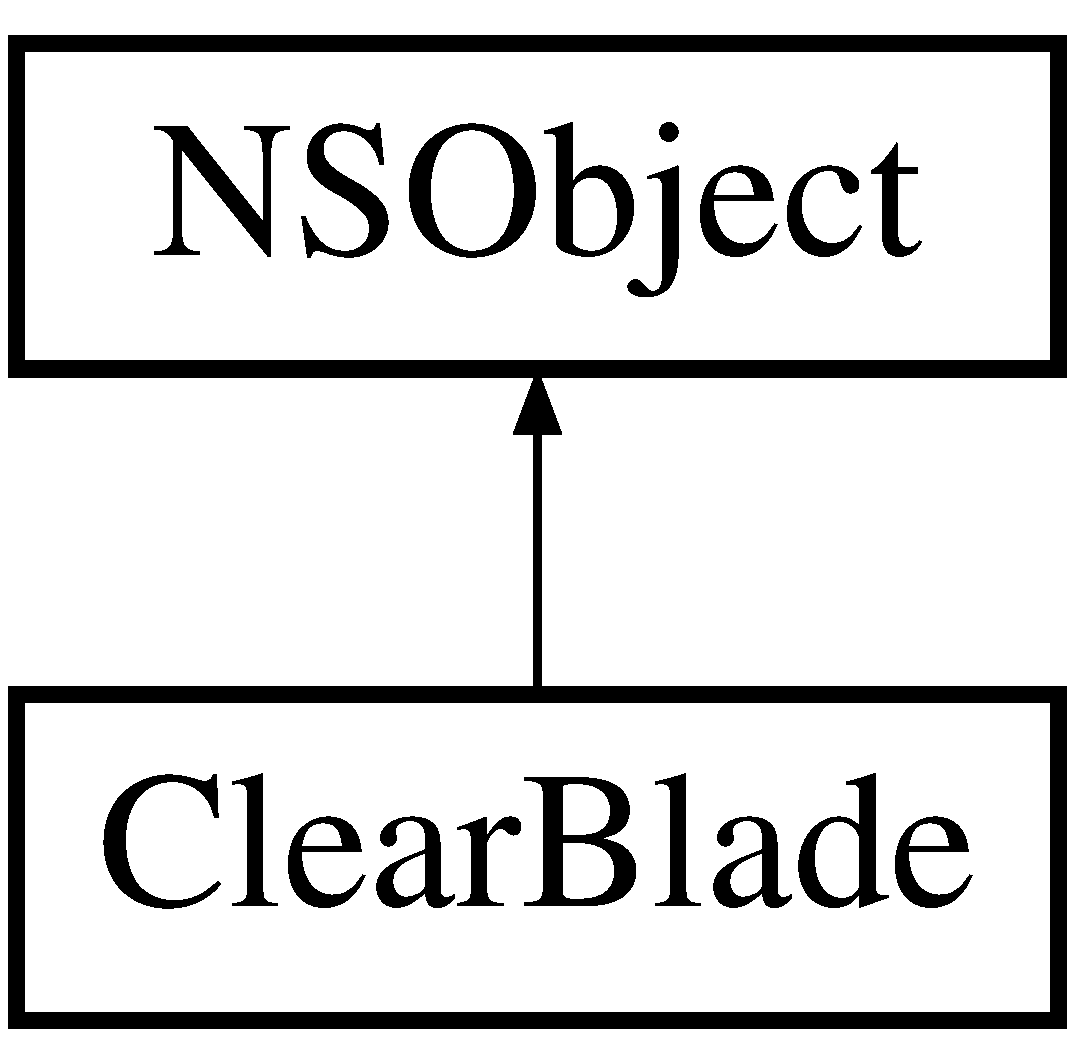
\includegraphics[height=2.000000cm]{interface_clear_blade}
\end{center}
\end{figure}
\subsection*{Instance Methods}
\begin{DoxyCompactItemize}
\item 
(void) -\/ \hyperlink{interface_clear_blade_a4a2da5ca59acd23e44d0f793e9eb778b}{log\+Error\+:}
\item 
(void) -\/ \hyperlink{interface_clear_blade_aa1d4699543bf38e300b5b0ad256c44c2}{log\+Warning\+:}
\item 
(void) -\/ \hyperlink{interface_clear_blade_ada4ef00171405d7247b1d07d3a3e70f6}{log\+Debug\+:}
\item 
(void) -\/ \hyperlink{interface_clear_blade_a03f35439a4d2b9908872cfdfbd50a0b5}{log\+Extra\+:}
\item 
(int) -\/ \hyperlink{interface_clear_blade_acdf4d6feb5a40c60be3b4ed0846d52e5}{generate\+I\+D}
\end{DoxyCompactItemize}
\subsection*{Class Methods}
\begin{DoxyCompactItemize}
\item 
(instancetype) + \hyperlink{interface_clear_blade_accced1239f531de87d166d617a021673}{settings}
\item 
(instancetype) + \hyperlink{interface_clear_blade_a234fefa317e73d46768506a34a89e5fa}{init\+Settings\+Sync\+With\+System\+Key\+:with\+System\+Secret\+:with\+Options\+:with\+Error\+:}
\item 
(void) + \hyperlink{interface_clear_blade_a76b3d3e815239c17dba4f858e774bcab}{init\+Settings\+With\+System\+Key\+:with\+System\+Secret\+:with\+Options\+:with\+Success\+Callback\+:with\+Error\+Callback\+:}
\end{DoxyCompactItemize}
\subsection*{Properties}
\begin{DoxyCompactItemize}
\item 
N\+S\+String $\ast$ \hyperlink{interface_clear_blade_aab0eaf0d5cb8cabae0889b19230859b5}{system\+Key}
\item 
N\+S\+String $\ast$ \hyperlink{interface_clear_blade_ac86550adaf64238807f4bc536af7d1d0}{system\+Secret}
\item 
N\+S\+String $\ast$ \hyperlink{interface_clear_blade_a254d692b3e85e4d33a4518e9ff9e4f40}{server\+Address}
\item 
N\+S\+U\+R\+L $\ast$ \hyperlink{interface_clear_blade_a6d90355650360ef27ac6aad5f3df2a7b}{messaging\+Address}
\item 
C\+B\+Message\+Client\+Quality \hyperlink{interface_clear_blade_a886dc9ea49818af85910b4373f95096b}{messaging\+Default\+Qo\+S}
\item 
\hyperlink{interface_c_b_user}{C\+B\+User} $\ast$ \hyperlink{interface_clear_blade_a2c5ec6113244b327a374c1f939efbce5}{main\+User}
\item 
C\+B\+Logging\+Level \hyperlink{interface_clear_blade_a63988be37c99a5e90c91b89be9106a5d}{logging\+Level}
\end{DoxyCompactItemize}


\subsection{Detailed Description}
Encapsulates all the global configuration for the \hyperlink{interface_clear_blade}{Clear\+Blade} A\+P\+I 

\subsection{Method Documentation}
\hypertarget{interface_clear_blade_acdf4d6feb5a40c60be3b4ed0846d52e5}{\index{Clear\+Blade@{Clear\+Blade}!generate\+I\+D@{generate\+I\+D}}
\index{generate\+I\+D@{generate\+I\+D}!Clear\+Blade@{Clear\+Blade}}
\subsubsection[{generate\+I\+D}]{\setlength{\rightskip}{0pt plus 5cm}-\/ (int) generate\+I\+D 
\begin{DoxyParamCaption}
{}
\end{DoxyParamCaption}
}}\label{interface_clear_blade_acdf4d6feb5a40c60be3b4ed0846d52e5}
Generates an I\+D that's guaranteed to be unique for this instance of \hyperlink{interface_clear_blade}{Clear\+Blade} Settings \hypertarget{interface_clear_blade_a234fefa317e73d46768506a34a89e5fa}{\index{Clear\+Blade@{Clear\+Blade}!init\+Settings\+Sync\+With\+System\+Key\+:with\+System\+Secret\+:with\+Options\+:with\+Error\+:@{init\+Settings\+Sync\+With\+System\+Key\+:with\+System\+Secret\+:with\+Options\+:with\+Error\+:}}
\index{init\+Settings\+Sync\+With\+System\+Key\+:with\+System\+Secret\+:with\+Options\+:with\+Error\+:@{init\+Settings\+Sync\+With\+System\+Key\+:with\+System\+Secret\+:with\+Options\+:with\+Error\+:}!Clear\+Blade@{Clear\+Blade}}
\subsubsection[{init\+Settings\+Sync\+With\+System\+Key\+:with\+System\+Secret\+:with\+Options\+:with\+Error\+:}]{\setlength{\rightskip}{0pt plus 5cm}+ (instancetype) init\+Settings\+Sync\+With\+System\+Key\+: 
\begin{DoxyParamCaption}
\item[{(N\+S\+String $\ast$)}]{key}
\item[{withSystemSecret:(N\+S\+String $\ast$)}]{secret}
\item[{withOptions:(N\+S\+Dictionary $\ast$)}]{options}
\item[{withError:(N\+S\+Error $\ast$$\ast$)}]{error}
\end{DoxyParamCaption}
}}\label{interface_clear_blade_a234fefa317e73d46768506a34a89e5fa}
Initializes settings synchronously with default settings. Also initializes with an anonymous user. 
\begin{DoxyParams}{Parameters}
{\em key} & The System Key. \\
\hline
{\em secret} & The System Secret. \\
\hline
{\em error} & Is set if the \hyperlink{interface_clear_blade}{Clear\+Blade} settings fails to initialize \\
\hline
\end{DoxyParams}
\begin{DoxyReturn}{Returns}
The newly created Settings object 
\end{DoxyReturn}
\hypertarget{interface_clear_blade_a76b3d3e815239c17dba4f858e774bcab}{\index{Clear\+Blade@{Clear\+Blade}!init\+Settings\+With\+System\+Key\+:with\+System\+Secret\+:with\+Options\+:with\+Success\+Callback\+:with\+Error\+Callback\+:@{init\+Settings\+With\+System\+Key\+:with\+System\+Secret\+:with\+Options\+:with\+Success\+Callback\+:with\+Error\+Callback\+:}}
\index{init\+Settings\+With\+System\+Key\+:with\+System\+Secret\+:with\+Options\+:with\+Success\+Callback\+:with\+Error\+Callback\+:@{init\+Settings\+With\+System\+Key\+:with\+System\+Secret\+:with\+Options\+:with\+Success\+Callback\+:with\+Error\+Callback\+:}!Clear\+Blade@{Clear\+Blade}}
\subsubsection[{init\+Settings\+With\+System\+Key\+:with\+System\+Secret\+:with\+Options\+:with\+Success\+Callback\+:with\+Error\+Callback\+:}]{\setlength{\rightskip}{0pt plus 5cm}+ (void) init\+Settings\+With\+System\+Key\+: 
\begin{DoxyParamCaption}
\item[{(N\+S\+String $\ast$)}]{key}
\item[{withSystemSecret:(N\+S\+String $\ast$)}]{secret}
\item[{withOptions:(N\+S\+Dictionary $\ast$)}]{options}
\item[{withSuccessCallback:(Clear\+Blade\+Settings\+Success\+Callback)}]{success\+Callback}
\item[{withErrorCallback:(Clear\+Blade\+Settings\+Error\+Callback)}]{error\+Callback}
\end{DoxyParamCaption}
}}\label{interface_clear_blade_a76b3d3e815239c17dba4f858e774bcab}
Initializes settings asynchronously with default settings. Also initializes with an anonymous user. 
\begin{DoxyParams}{Parameters}
{\em key} & The System Key. \\
\hline
{\em secret} & The System Secret. \\
\hline
{\em success\+Callback} & The callback for when settings successfully initializes. \\
\hline
{\em error\+Callback} & The callback for when settings fails to initialize for whatever reason \\
\hline
\end{DoxyParams}
\hypertarget{interface_clear_blade_ada4ef00171405d7247b1d07d3a3e70f6}{\index{Clear\+Blade@{Clear\+Blade}!log\+Debug\+:@{log\+Debug\+:}}
\index{log\+Debug\+:@{log\+Debug\+:}!Clear\+Blade@{Clear\+Blade}}
\subsubsection[{log\+Debug\+:}]{\setlength{\rightskip}{0pt plus 5cm}-\/ (void) log\+Debug\+: 
\begin{DoxyParamCaption}
\item[{(N\+S\+String $\ast$)}]{debug}
\item[{,}]{...}
\end{DoxyParamCaption}
}}\label{interface_clear_blade_ada4ef00171405d7247b1d07d3a3e70f6}
Logs a debug statement as filtered by the logging\+Level setting \hypertarget{interface_clear_blade_a4a2da5ca59acd23e44d0f793e9eb778b}{\index{Clear\+Blade@{Clear\+Blade}!log\+Error\+:@{log\+Error\+:}}
\index{log\+Error\+:@{log\+Error\+:}!Clear\+Blade@{Clear\+Blade}}
\subsubsection[{log\+Error\+:}]{\setlength{\rightskip}{0pt plus 5cm}-\/ (void) log\+Error\+: 
\begin{DoxyParamCaption}
\item[{(N\+S\+String $\ast$)}]{error}
\item[{,}]{...}
\end{DoxyParamCaption}
}}\label{interface_clear_blade_a4a2da5ca59acd23e44d0f793e9eb778b}
Logs an error as filtered by the logging\+Level setting \hypertarget{interface_clear_blade_a03f35439a4d2b9908872cfdfbd50a0b5}{\index{Clear\+Blade@{Clear\+Blade}!log\+Extra\+:@{log\+Extra\+:}}
\index{log\+Extra\+:@{log\+Extra\+:}!Clear\+Blade@{Clear\+Blade}}
\subsubsection[{log\+Extra\+:}]{\setlength{\rightskip}{0pt plus 5cm}-\/ (void) log\+Extra\+: 
\begin{DoxyParamCaption}
\item[{(N\+S\+String $\ast$)}]{extra}
\item[{,}]{...}
\end{DoxyParamCaption}
}}\label{interface_clear_blade_a03f35439a4d2b9908872cfdfbd50a0b5}
Logs a extra data as filtered by the logging\+Level setting \hypertarget{interface_clear_blade_aa1d4699543bf38e300b5b0ad256c44c2}{\index{Clear\+Blade@{Clear\+Blade}!log\+Warning\+:@{log\+Warning\+:}}
\index{log\+Warning\+:@{log\+Warning\+:}!Clear\+Blade@{Clear\+Blade}}
\subsubsection[{log\+Warning\+:}]{\setlength{\rightskip}{0pt plus 5cm}-\/ (void) log\+Warning\+: 
\begin{DoxyParamCaption}
\item[{(N\+S\+String $\ast$)}]{warning}
\item[{,}]{...}
\end{DoxyParamCaption}
}}\label{interface_clear_blade_aa1d4699543bf38e300b5b0ad256c44c2}
Logs a warning as filtered by the logging\+Level setting \hypertarget{interface_clear_blade_accced1239f531de87d166d617a021673}{\index{Clear\+Blade@{Clear\+Blade}!settings@{settings}}
\index{settings@{settings}!Clear\+Blade@{Clear\+Blade}}
\subsubsection[{settings}]{\setlength{\rightskip}{0pt plus 5cm}+ (instancetype) settings 
\begin{DoxyParamCaption}
{}
\end{DoxyParamCaption}
}}\label{interface_clear_blade_accced1239f531de87d166d617a021673}
The global settings used by queries by default 

\subsection{Property Documentation}
\hypertarget{interface_clear_blade_a63988be37c99a5e90c91b89be9106a5d}{\index{Clear\+Blade@{Clear\+Blade}!logging\+Level@{logging\+Level}}
\index{logging\+Level@{logging\+Level}!Clear\+Blade@{Clear\+Blade}}
\subsubsection[{logging\+Level}]{\setlength{\rightskip}{0pt plus 5cm}-\/ (C\+B\+Logging\+Level) logging\+Level\hspace{0.3cm}{\ttfamily [read]}, {\ttfamily [write]}, {\ttfamily [atomic]}, {\ttfamily [assign]}}}\label{interface_clear_blade_a63988be37c99a5e90c91b89be9106a5d}
The Logging level the A\+P\+I uses. Defaults to C\+B\+\_\+\+L\+O\+G\+\_\+\+W\+A\+R\+N \hypertarget{interface_clear_blade_a2c5ec6113244b327a374c1f939efbce5}{\index{Clear\+Blade@{Clear\+Blade}!main\+User@{main\+User}}
\index{main\+User@{main\+User}!Clear\+Blade@{Clear\+Blade}}
\subsubsection[{main\+User}]{\setlength{\rightskip}{0pt plus 5cm}-\/ ({\bf C\+B\+User}$\ast$) main\+User\hspace{0.3cm}{\ttfamily [read]}, {\ttfamily [write]}, {\ttfamily [atomic]}, {\ttfamily [strong]}}}\label{interface_clear_blade_a2c5ec6113244b327a374c1f939efbce5}
The Main User of the app. Can be modified at runtime to change main users \hypertarget{interface_clear_blade_a6d90355650360ef27ac6aad5f3df2a7b}{\index{Clear\+Blade@{Clear\+Blade}!messaging\+Address@{messaging\+Address}}
\index{messaging\+Address@{messaging\+Address}!Clear\+Blade@{Clear\+Blade}}
\subsubsection[{messaging\+Address}]{\setlength{\rightskip}{0pt plus 5cm}-\/ (N\+S\+U\+R\+L$\ast$) messaging\+Address\hspace{0.3cm}{\ttfamily [read]}, {\ttfamily [atomic]}, {\ttfamily [assign]}}}\label{interface_clear_blade_a6d90355650360ef27ac6aad5f3df2a7b}
The Address for the Platform messaging service \hypertarget{interface_clear_blade_a886dc9ea49818af85910b4373f95096b}{\index{Clear\+Blade@{Clear\+Blade}!messaging\+Default\+Qo\+S@{messaging\+Default\+Qo\+S}}
\index{messaging\+Default\+Qo\+S@{messaging\+Default\+Qo\+S}!Clear\+Blade@{Clear\+Blade}}
\subsubsection[{messaging\+Default\+Qo\+S}]{\setlength{\rightskip}{0pt plus 5cm}-\/ (C\+B\+Message\+Client\+Quality) messaging\+Default\+Qo\+S\hspace{0.3cm}{\ttfamily [read]}, {\ttfamily [atomic]}, {\ttfamily [assign]}}}\label{interface_clear_blade_a886dc9ea49818af85910b4373f95096b}
The Default quality of service to use for messaging clients \hypertarget{interface_clear_blade_a254d692b3e85e4d33a4518e9ff9e4f40}{\index{Clear\+Blade@{Clear\+Blade}!server\+Address@{server\+Address}}
\index{server\+Address@{server\+Address}!Clear\+Blade@{Clear\+Blade}}
\subsubsection[{server\+Address}]{\setlength{\rightskip}{0pt plus 5cm}-\/ (N\+S\+String$\ast$) server\+Address\hspace{0.3cm}{\ttfamily [read]}, {\ttfamily [atomic]}, {\ttfamily [assign]}}}\label{interface_clear_blade_a254d692b3e85e4d33a4518e9ff9e4f40}
The Address for the Platform Data service \hypertarget{interface_clear_blade_aab0eaf0d5cb8cabae0889b19230859b5}{\index{Clear\+Blade@{Clear\+Blade}!system\+Key@{system\+Key}}
\index{system\+Key@{system\+Key}!Clear\+Blade@{Clear\+Blade}}
\subsubsection[{system\+Key}]{\setlength{\rightskip}{0pt plus 5cm}-\/ (N\+S\+String$\ast$) system\+Key\hspace{0.3cm}{\ttfamily [read]}, {\ttfamily [atomic]}, {\ttfamily [assign]}}}\label{interface_clear_blade_aab0eaf0d5cb8cabae0889b19230859b5}
The System Key used throughout the A\+P\+I \hypertarget{interface_clear_blade_ac86550adaf64238807f4bc536af7d1d0}{\index{Clear\+Blade@{Clear\+Blade}!system\+Secret@{system\+Secret}}
\index{system\+Secret@{system\+Secret}!Clear\+Blade@{Clear\+Blade}}
\subsubsection[{system\+Secret}]{\setlength{\rightskip}{0pt plus 5cm}-\/ (N\+S\+String$\ast$) system\+Secret\hspace{0.3cm}{\ttfamily [read]}, {\ttfamily [atomic]}, {\ttfamily [assign]}}}\label{interface_clear_blade_ac86550adaf64238807f4bc536af7d1d0}
The System Secret used throughout the A\+P\+I 

The documentation for this class was generated from the following file\+:\begin{DoxyCompactItemize}
\item 
Clear\+Blade\+A\+P\+I/Clear\+Blade.\+h\end{DoxyCompactItemize}

\hypertarget{interface_m_q_t_t_client}{\section{M\-Q\-T\-T\-Client Class Reference}
\label{interface_m_q_t_t_client}\index{M\-Q\-T\-T\-Client@{M\-Q\-T\-T\-Client}}
}
Inheritance diagram for M\-Q\-T\-T\-Client\-:\begin{figure}[H]
\begin{center}
\leavevmode
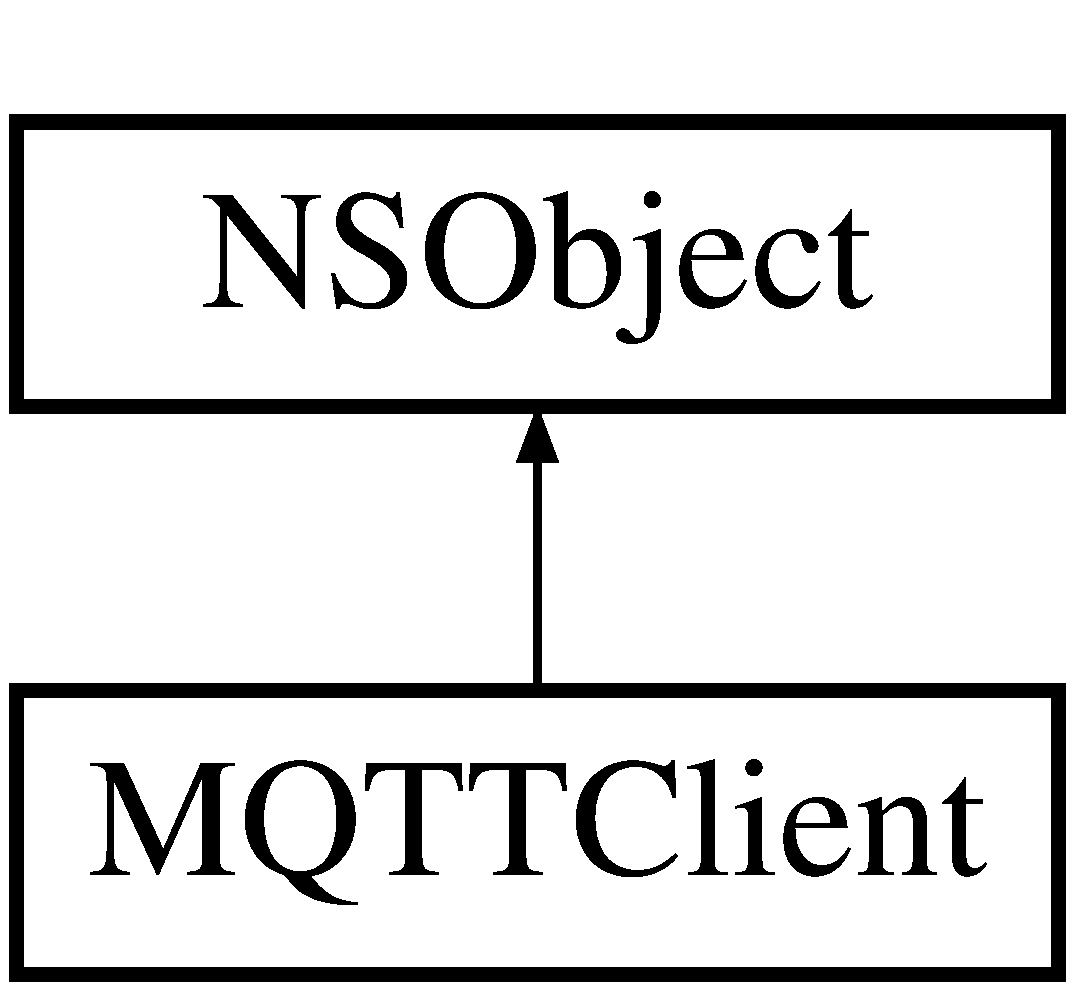
\includegraphics[height=2.000000cm]{interface_m_q_t_t_client}
\end{center}
\end{figure}
\subsection*{Instance Methods}
\begin{DoxyCompactItemize}
\item 
(\hyperlink{interface_m_q_t_t_client}{M\-Q\-T\-T\-Client} $\ast$) -\/ \hyperlink{interface_m_q_t_t_client_a2ca50eb85a638fe1dd3415eaa55b79eb}{init\-With\-Client\-Id\-:}
\item 
(void) -\/ \hyperlink{interface_m_q_t_t_client_afd942b93568e259fba6b22abec4bea59}{set\-Message\-Retry\-:}
\item 
(void) -\/ \hyperlink{interface_m_q_t_t_client_a209e35ab865030b42518b0f94713694a}{connect}
\item 
(void) -\/ \hyperlink{interface_m_q_t_t_client_affe3571b6b972fb3f41ceea7778de723}{connect\-To\-Host\-:}
\item 
(void) -\/ \hyperlink{interface_m_q_t_t_client_a8a2180a68956d6a897f068994e5c8864}{reconnect}
\item 
(void) -\/ \hyperlink{interface_m_q_t_t_client_a5da21136f56343f0db9dba70e0384ba9}{disconnect}
\item 
(void) -\/ \hyperlink{interface_m_q_t_t_client_a8af6c4267519439b5d0b2eb91bc0eb8d}{set\-Will\-:to\-Topic\-:with\-Qos\-:retain\-:}
\item 
(void) -\/ \hyperlink{interface_m_q_t_t_client_a70b2a3eb06df7dc5f12b550d4df3a28a}{clear\-Will}
\item 
(void) -\/ \hyperlink{interface_m_q_t_t_client_adad97fb0b40b931c232de1b691155fbd}{publish\-String\-:to\-Topic\-:with\-Qos\-:retain\-:}
\item 
(void) -\/ \hyperlink{interface_m_q_t_t_client_aa49277b1d3806e73cc16a1aa13a6ecfc}{subscribe\-:}
\item 
(void) -\/ \hyperlink{interface_m_q_t_t_client_a8d389ce309a69c1049caf92ed2c70e59}{subscribe\-:with\-Qos\-:}
\item 
(void) -\/ \hyperlink{interface_m_q_t_t_client_a712c2fe6afed9d57794c81b483238ecc}{unsubscribe\-:}
\item 
\hypertarget{interface_m_q_t_t_client_aa51b52a52ad834465ac4e0ae27997895}{(void) -\/ {\bfseries loop\-:}}\label{interface_m_q_t_t_client_aa51b52a52ad834465ac4e0ae27997895}

\end{DoxyCompactItemize}
\subsection*{Class Methods}
\begin{DoxyCompactItemize}
\item 
\hypertarget{interface_m_q_t_t_client_addc8362ee9e927f944c604daf5f7e0c7}{(void) + {\bfseries initialize}}\label{interface_m_q_t_t_client_addc8362ee9e927f944c604daf5f7e0c7}

\item 
\hypertarget{interface_m_q_t_t_client_a28d3f42ae2595214b2c40794ca638c45}{(N\-S\-String $\ast$) + {\bfseries version}}\label{interface_m_q_t_t_client_a28d3f42ae2595214b2c40794ca638c45}

\end{DoxyCompactItemize}
\subsection*{Protected Attributes}
\begin{DoxyCompactItemize}
\item 
\hypertarget{interface_m_q_t_t_client_ae4f553d3d5b3f96833631fa71d089cae}{struct mosquitto $\ast$ {\bfseries mosq}}\label{interface_m_q_t_t_client_ae4f553d3d5b3f96833631fa71d089cae}

\item 
\hypertarget{interface_m_q_t_t_client_a947472d48ef128a407c579f3f03b6bb6}{N\-S\-Timer $\ast$ {\bfseries timer}}\label{interface_m_q_t_t_client_a947472d48ef128a407c579f3f03b6bb6}

\end{DoxyCompactItemize}
\subsection*{Properties}
\begin{DoxyCompactItemize}
\item 
N\-S\-String $\ast$ \hyperlink{interface_m_q_t_t_client_a1f617c2783f5f49fe0eade772b848330}{host}
\item 
unsigned short \hyperlink{interface_m_q_t_t_client_a1d5b24d0ebc1a18fa8cb85a48381513e}{port}
\item 
N\-S\-String $\ast$ \hyperlink{interface_m_q_t_t_client_aba20ca92199c2b75f3993468db429aed}{username}
\item 
N\-S\-String $\ast$ \hyperlink{interface_m_q_t_t_client_adb44dfa2630f0ac31524a0823c1f00f4}{password}
\item 
unsigned short \hyperlink{interface_m_q_t_t_client_a39d172ccd9c5f7c4d7927a547c496d6e}{keep\-Alive}
\item 
B\-O\-O\-L \hyperlink{interface_m_q_t_t_client_a097920820d62efef6d17060fbabf3b09}{clean\-Session}
\item 
id$<$ \hyperlink{protocol_m_q_t_t_client_delegate-p}{M\-Q\-T\-T\-Client\-Delegate} $>$ \hyperlink{interface_m_q_t_t_client_ae177aa16bf5c66e71db4c21820de7623}{delegate}
\end{DoxyCompactItemize}


\subsection{Method Documentation}
\hypertarget{interface_m_q_t_t_client_a70b2a3eb06df7dc5f12b550d4df3a28a}{\index{M\-Q\-T\-T\-Client@{M\-Q\-T\-T\-Client}!clear\-Will@{clear\-Will}}
\index{clear\-Will@{clear\-Will}!MQTTClient@{M\-Q\-T\-T\-Client}}
\subsubsection[{clear\-Will}]{\setlength{\rightskip}{0pt plus 5cm}-\/ (void) clear\-Will 
\begin{DoxyParamCaption}
{}
\end{DoxyParamCaption}
}}\label{interface_m_q_t_t_client_a70b2a3eb06df7dc5f12b550d4df3a28a}
Clears the will that was set with set\-Will(). \hypertarget{interface_m_q_t_t_client_a209e35ab865030b42518b0f94713694a}{\index{M\-Q\-T\-T\-Client@{M\-Q\-T\-T\-Client}!connect@{connect}}
\index{connect@{connect}!MQTTClient@{M\-Q\-T\-T\-Client}}
\subsubsection[{connect}]{\setlength{\rightskip}{0pt plus 5cm}-\/ (void) connect 
\begin{DoxyParamCaption}
{}
\end{DoxyParamCaption}
}}\label{interface_m_q_t_t_client_a209e35ab865030b42518b0f94713694a}
Connects to the host designated if the host has already been set. \hypertarget{interface_m_q_t_t_client_affe3571b6b972fb3f41ceea7778de723}{\index{M\-Q\-T\-T\-Client@{M\-Q\-T\-T\-Client}!connect\-To\-Host\-:@{connect\-To\-Host\-:}}
\index{connect\-To\-Host\-:@{connect\-To\-Host\-:}!MQTTClient@{M\-Q\-T\-T\-Client}}
\subsubsection[{connect\-To\-Host\-:}]{\setlength{\rightskip}{0pt plus 5cm}-\/ (void) connect\-To\-Host\-: 
\begin{DoxyParamCaption}
\item[{(N\-S\-String$\ast$)}]{host}
\end{DoxyParamCaption}
}}\label{interface_m_q_t_t_client_affe3571b6b972fb3f41ceea7778de723}
Connects to the given host. 
\begin{DoxyParams}{Parameters}
{\em host} & String that represents the host address. \\
\hline
\end{DoxyParams}
\hypertarget{interface_m_q_t_t_client_a5da21136f56343f0db9dba70e0384ba9}{\index{M\-Q\-T\-T\-Client@{M\-Q\-T\-T\-Client}!disconnect@{disconnect}}
\index{disconnect@{disconnect}!MQTTClient@{M\-Q\-T\-T\-Client}}
\subsubsection[{disconnect}]{\setlength{\rightskip}{0pt plus 5cm}-\/ (void) disconnect 
\begin{DoxyParamCaption}
{}
\end{DoxyParamCaption}
}}\label{interface_m_q_t_t_client_a5da21136f56343f0db9dba70e0384ba9}
Disconnect from the host. \hypertarget{interface_m_q_t_t_client_a2ca50eb85a638fe1dd3415eaa55b79eb}{\index{M\-Q\-T\-T\-Client@{M\-Q\-T\-T\-Client}!init\-With\-Client\-Id\-:@{init\-With\-Client\-Id\-:}}
\index{init\-With\-Client\-Id\-:@{init\-With\-Client\-Id\-:}!MQTTClient@{M\-Q\-T\-T\-Client}}
\subsubsection[{init\-With\-Client\-Id\-:}]{\setlength{\rightskip}{0pt plus 5cm}-\/ ({\bf M\-Q\-T\-T\-Client} $\ast$) init\-With\-Client\-Id\-: 
\begin{DoxyParamCaption}
\item[{(N\-S\-String $\ast$)}]{client\-Id}
\end{DoxyParamCaption}
}}\label{interface_m_q_t_t_client_a2ca50eb85a638fe1dd3415eaa55b79eb}
Initalize a new \hyperlink{interface_m_q_t_t_client}{M\-Q\-T\-T\-Client} object with a client\-I\-D 
\begin{DoxyParams}{Parameters}
{\em client\-Id} & String that represents the client I\-D \\
\hline
\end{DoxyParams}
\begin{DoxyReturn}{Returns}
a newly initialized \hyperlink{interface_m_q_t_t_client}{M\-Q\-T\-T\-Client} 
\end{DoxyReturn}
\hypertarget{interface_m_q_t_t_client_adad97fb0b40b931c232de1b691155fbd}{\index{M\-Q\-T\-T\-Client@{M\-Q\-T\-T\-Client}!publish\-String\-:to\-Topic\-:with\-Qos\-:retain\-:@{publish\-String\-:to\-Topic\-:with\-Qos\-:retain\-:}}
\index{publish\-String\-:to\-Topic\-:with\-Qos\-:retain\-:@{publish\-String\-:to\-Topic\-:with\-Qos\-:retain\-:}!MQTTClient@{M\-Q\-T\-T\-Client}}
\subsubsection[{publish\-String\-:to\-Topic\-:with\-Qos\-:retain\-:}]{\setlength{\rightskip}{0pt plus 5cm}-\/ (void) publish\-String\-: 
\begin{DoxyParamCaption}
\item[{(N\-S\-String $\ast$)}]{payload}
\item[{toTopic:(N\-S\-String $\ast$)}]{topic}
\item[{withQos:(N\-S\-U\-Integer)}]{qos}
\item[{retain:(B\-O\-O\-L)}]{retain}
\end{DoxyParamCaption}
}}\label{interface_m_q_t_t_client_adad97fb0b40b931c232de1b691155fbd}
Publishes a string to the host on a given topic 
\begin{DoxyParams}{Parameters}
{\em payload} & String that holds the message to be sent \\
\hline
{\em topic} & String that represents the topic to which the message is sent \\
\hline
{\em qos} & N\-S\-U\-Integer that represents the quality of service level that the message will be sent with \\
\hline
{\em retain} & B\-O\-O\-L that flags the message to be retained or not \\
\hline
\end{DoxyParams}
\hypertarget{interface_m_q_t_t_client_a8a2180a68956d6a897f068994e5c8864}{\index{M\-Q\-T\-T\-Client@{M\-Q\-T\-T\-Client}!reconnect@{reconnect}}
\index{reconnect@{reconnect}!MQTTClient@{M\-Q\-T\-T\-Client}}
\subsubsection[{reconnect}]{\setlength{\rightskip}{0pt plus 5cm}-\/ (void) reconnect 
\begin{DoxyParamCaption}
{}
\end{DoxyParamCaption}
}}\label{interface_m_q_t_t_client_a8a2180a68956d6a897f068994e5c8864}
Disconnect from the host and establish a new connection. \hypertarget{interface_m_q_t_t_client_afd942b93568e259fba6b22abec4bea59}{\index{M\-Q\-T\-T\-Client@{M\-Q\-T\-T\-Client}!set\-Message\-Retry\-:@{set\-Message\-Retry\-:}}
\index{set\-Message\-Retry\-:@{set\-Message\-Retry\-:}!MQTTClient@{M\-Q\-T\-T\-Client}}
\subsubsection[{set\-Message\-Retry\-:}]{\setlength{\rightskip}{0pt plus 5cm}-\/ (void) set\-Message\-Retry\-: 
\begin{DoxyParamCaption}
\item[{(N\-S\-U\-Integer)}]{seconds}
\end{DoxyParamCaption}
}}\label{interface_m_q_t_t_client_afd942b93568e259fba6b22abec4bea59}
Sets how often the message will retry. 
\begin{DoxyParams}{Parameters}
{\em seconds} & N\-S\-U\-Integer that represent the amount of time between retries. \\
\hline
\end{DoxyParams}
\hypertarget{interface_m_q_t_t_client_a8af6c4267519439b5d0b2eb91bc0eb8d}{\index{M\-Q\-T\-T\-Client@{M\-Q\-T\-T\-Client}!set\-Will\-:to\-Topic\-:with\-Qos\-:retain\-:@{set\-Will\-:to\-Topic\-:with\-Qos\-:retain\-:}}
\index{set\-Will\-:to\-Topic\-:with\-Qos\-:retain\-:@{set\-Will\-:to\-Topic\-:with\-Qos\-:retain\-:}!MQTTClient@{M\-Q\-T\-T\-Client}}
\subsubsection[{set\-Will\-:to\-Topic\-:with\-Qos\-:retain\-:}]{\setlength{\rightskip}{0pt plus 5cm}-\/ (void) set\-Will\-: 
\begin{DoxyParamCaption}
\item[{(N\-S\-String $\ast$)}]{payload}
\item[{toTopic:(N\-S\-String $\ast$)}]{will\-Topic}
\item[{withQos:(N\-S\-U\-Integer)}]{will\-Qos}
\item[{retain:(B\-O\-O\-L)}]{retain}
\end{DoxyParamCaption}
}}\label{interface_m_q_t_t_client_a8af6c4267519439b5d0b2eb91bc0eb8d}
Message to be sent upon disconnect 
\begin{DoxyParams}{Parameters}
{\em payload} & String that holds the message to be sent \\
\hline
{\em will\-Topic} & String that represents the topic to which the Will message is sent \\
\hline
{\em will\-Qos} & N\-S\-U\-Integer that represents the quality of service level that the message will be sent with \\
\hline
{\em retain} & B\-O\-O\-L that flags the message to be retained or not \\
\hline
\end{DoxyParams}
\hypertarget{interface_m_q_t_t_client_aa49277b1d3806e73cc16a1aa13a6ecfc}{\index{M\-Q\-T\-T\-Client@{M\-Q\-T\-T\-Client}!subscribe\-:@{subscribe\-:}}
\index{subscribe\-:@{subscribe\-:}!MQTTClient@{M\-Q\-T\-T\-Client}}
\subsubsection[{subscribe\-:}]{\setlength{\rightskip}{0pt plus 5cm}-\/ (void) subscribe\-: 
\begin{DoxyParamCaption}
\item[{(N\-S\-String $\ast$)}]{topic}
\end{DoxyParamCaption}
}}\label{interface_m_q_t_t_client_aa49277b1d3806e73cc16a1aa13a6ecfc}
Subscribes to the given topic to receive messages sent to that topic 
\begin{DoxyParams}{Parameters}
{\em topic} & String that represents the topic to be listened on \\
\hline
\end{DoxyParams}
\hypertarget{interface_m_q_t_t_client_a8d389ce309a69c1049caf92ed2c70e59}{\index{M\-Q\-T\-T\-Client@{M\-Q\-T\-T\-Client}!subscribe\-:with\-Qos\-:@{subscribe\-:with\-Qos\-:}}
\index{subscribe\-:with\-Qos\-:@{subscribe\-:with\-Qos\-:}!MQTTClient@{M\-Q\-T\-T\-Client}}
\subsubsection[{subscribe\-:with\-Qos\-:}]{\setlength{\rightskip}{0pt plus 5cm}-\/ (void) {\bf subscribe\-:} 
\begin{DoxyParamCaption}
\item[{(N\-S\-String $\ast$)}]{topic}
\item[{withQos:(N\-S\-U\-Integer)}]{qos}
\end{DoxyParamCaption}
}}\label{interface_m_q_t_t_client_a8d389ce309a69c1049caf92ed2c70e59}
Subscribes to the given topic to receive messages sent to that topic with the given Q\-O\-S 
\begin{DoxyParams}{Parameters}
{\em topic} & String that represents the topic to be listened on \\
\hline
{\em qos} & N\-S\-U\-Integer that represents the quality of service level that the message will be recieved with \\
\hline
\end{DoxyParams}
\hypertarget{interface_m_q_t_t_client_a712c2fe6afed9d57794c81b483238ecc}{\index{M\-Q\-T\-T\-Client@{M\-Q\-T\-T\-Client}!unsubscribe\-:@{unsubscribe\-:}}
\index{unsubscribe\-:@{unsubscribe\-:}!MQTTClient@{M\-Q\-T\-T\-Client}}
\subsubsection[{unsubscribe\-:}]{\setlength{\rightskip}{0pt plus 5cm}-\/ (void) unsubscribe\-: 
\begin{DoxyParamCaption}
\item[{(N\-S\-String $\ast$)}]{topic}
\end{DoxyParamCaption}
}}\label{interface_m_q_t_t_client_a712c2fe6afed9d57794c81b483238ecc}
Unsubscibes from the given topic 
\begin{DoxyParams}{Parameters}
{\em topic} & String that represents the topic from which to be unsubscribed \\
\hline
\end{DoxyParams}


\subsection{Property Documentation}
\hypertarget{interface_m_q_t_t_client_a097920820d62efef6d17060fbabf3b09}{\index{M\-Q\-T\-T\-Client@{M\-Q\-T\-T\-Client}!clean\-Session@{clean\-Session}}
\index{clean\-Session@{clean\-Session}!MQTTClient@{M\-Q\-T\-T\-Client}}
\subsubsection[{clean\-Session}]{\setlength{\rightskip}{0pt plus 5cm}-\/ (B\-O\-O\-L) clean\-Session\hspace{0.3cm}{\ttfamily [read]}, {\ttfamily [write]}, {\ttfamily [atomic]}, {\ttfamily [assign]}}}\label{interface_m_q_t_t_client_a097920820d62efef6d17060fbabf3b09}
Boolean to flag a clean session. \hypertarget{interface_m_q_t_t_client_ae177aa16bf5c66e71db4c21820de7623}{\index{M\-Q\-T\-T\-Client@{M\-Q\-T\-T\-Client}!delegate@{delegate}}
\index{delegate@{delegate}!MQTTClient@{M\-Q\-T\-T\-Client}}
\subsubsection[{delegate}]{\setlength{\rightskip}{0pt plus 5cm}-\/ (id$<${\bf M\-Q\-T\-T\-Client\-Delegate}$>$) delegate\hspace{0.3cm}{\ttfamily [read]}, {\ttfamily [write]}, {\ttfamily [atomic]}, {\ttfamily [assign]}}}\label{interface_m_q_t_t_client_ae177aa16bf5c66e71db4c21820de7623}
Pointer to the delegate object that will handle messages when received. \hypertarget{interface_m_q_t_t_client_a1f617c2783f5f49fe0eade772b848330}{\index{M\-Q\-T\-T\-Client@{M\-Q\-T\-T\-Client}!host@{host}}
\index{host@{host}!MQTTClient@{M\-Q\-T\-T\-Client}}
\subsubsection[{host}]{\setlength{\rightskip}{0pt plus 5cm}-\/ (N\-S\-String $\ast$) host\hspace{0.3cm}{\ttfamily [read]}, {\ttfamily [write]}, {\ttfamily [atomic]}, {\ttfamily [retain]}}}\label{interface_m_q_t_t_client_a1f617c2783f5f49fe0eade772b848330}
The string that holds the host address. \hypertarget{interface_m_q_t_t_client_a39d172ccd9c5f7c4d7927a547c496d6e}{\index{M\-Q\-T\-T\-Client@{M\-Q\-T\-T\-Client}!keep\-Alive@{keep\-Alive}}
\index{keep\-Alive@{keep\-Alive}!MQTTClient@{M\-Q\-T\-T\-Client}}
\subsubsection[{keep\-Alive}]{\setlength{\rightskip}{0pt plus 5cm}-\/ (unsigned short) keep\-Alive\hspace{0.3cm}{\ttfamily [read]}, {\ttfamily [write]}, {\ttfamily [atomic]}, {\ttfamily [assign]}}}\label{interface_m_q_t_t_client_a39d172ccd9c5f7c4d7927a547c496d6e}
The amount of time to keep alive \hypertarget{interface_m_q_t_t_client_adb44dfa2630f0ac31524a0823c1f00f4}{\index{M\-Q\-T\-T\-Client@{M\-Q\-T\-T\-Client}!password@{password}}
\index{password@{password}!MQTTClient@{M\-Q\-T\-T\-Client}}
\subsubsection[{password}]{\setlength{\rightskip}{0pt plus 5cm}-\/ (N\-S\-String $\ast$) password\hspace{0.3cm}{\ttfamily [read]}, {\ttfamily [write]}, {\ttfamily [atomic]}, {\ttfamily [retain]}}}\label{interface_m_q_t_t_client_adb44dfa2630f0ac31524a0823c1f00f4}
The string that holds the password of the client. \hypertarget{interface_m_q_t_t_client_a1d5b24d0ebc1a18fa8cb85a48381513e}{\index{M\-Q\-T\-T\-Client@{M\-Q\-T\-T\-Client}!port@{port}}
\index{port@{port}!MQTTClient@{M\-Q\-T\-T\-Client}}
\subsubsection[{port}]{\setlength{\rightskip}{0pt plus 5cm}-\/ (unsigned short) port\hspace{0.3cm}{\ttfamily [read]}, {\ttfamily [write]}, {\ttfamily [atomic]}, {\ttfamily [assign]}}}\label{interface_m_q_t_t_client_a1d5b24d0ebc1a18fa8cb85a48381513e}
The port number of the host. \hypertarget{interface_m_q_t_t_client_aba20ca92199c2b75f3993468db429aed}{\index{M\-Q\-T\-T\-Client@{M\-Q\-T\-T\-Client}!username@{username}}
\index{username@{username}!MQTTClient@{M\-Q\-T\-T\-Client}}
\subsubsection[{username}]{\setlength{\rightskip}{0pt plus 5cm}-\/ (N\-S\-String $\ast$) username\hspace{0.3cm}{\ttfamily [read]}, {\ttfamily [write]}, {\ttfamily [atomic]}, {\ttfamily [retain]}}}\label{interface_m_q_t_t_client_aba20ca92199c2b75f3993468db429aed}
The string that holds the username of the client. 

The documentation for this class was generated from the following files\-:\begin{DoxyCompactItemize}
\item 
M\-Q\-T\-T\-Client.\-h\item 
M\-Q\-T\-T\-Client.\-m\end{DoxyCompactItemize}

\hypertarget{protocol_m_q_t_t_client_delegate-p}{\section{$<$M\-Q\-T\-T\-Client\-Delegate$>$ Protocol Reference}
\label{protocol_m_q_t_t_client_delegate-p}\index{$<$\-M\-Q\-T\-T\-Client\-Delegate$>$@{$<$\-M\-Q\-T\-T\-Client\-Delegate$>$}}
}
\subsection*{Instance Methods}
\begin{DoxyCompactItemize}
\item 
(void) -\/ \hyperlink{protocol_m_q_t_t_client_delegate-p_abb74a5596c9ad44a7052211b93e37cc9}{did\-Connect\-:}
\item 
(void) -\/ \hyperlink{protocol_m_q_t_t_client_delegate-p_af2c500a4d472477e679d645c5b27d85c}{did\-Disconnect}
\item 
(void) -\/ \hyperlink{protocol_m_q_t_t_client_delegate-p_ae779c7d4627f8aa3e154b42b76433884}{did\-Publish\-:}
\item 
(void) -\/ \hyperlink{protocol_m_q_t_t_client_delegate-p_a6222052eaf37f65f0b535daac93b917b}{did\-Receive\-Message\-:}
\item 
(void) -\/ \hyperlink{protocol_m_q_t_t_client_delegate-p_a1ace3cd8729f0f4ae0f0b4426005fbc6}{did\-Subscribe\-:granted\-Qos\-:}
\item 
(void) -\/ \hyperlink{protocol_m_q_t_t_client_delegate-p_a0413071b5250d70186de525049240038}{did\-Unsubscribe\-:}
\end{DoxyCompactItemize}


\subsection{Method Documentation}
\hypertarget{protocol_m_q_t_t_client_delegate-p_abb74a5596c9ad44a7052211b93e37cc9}{\index{M\-Q\-T\-T\-Client\-Delegate-\/p@{M\-Q\-T\-T\-Client\-Delegate-\/p}!did\-Connect\-:@{did\-Connect\-:}}
\index{did\-Connect\-:@{did\-Connect\-:}!MQTTClientDelegate-p@{M\-Q\-T\-T\-Client\-Delegate-\/p}}
\subsubsection[{did\-Connect\-:}]{\setlength{\rightskip}{0pt plus 5cm}-\/ (void) did\-Connect\-: 
\begin{DoxyParamCaption}
\item[{(N\-S\-U\-Integer)}]{code}
\end{DoxyParamCaption}
}}\label{protocol_m_q_t_t_client_delegate-p_abb74a5596c9ad44a7052211b93e37cc9}
Method that gets called upon successful connection 
\begin{DoxyParams}{Parameters}
{\em code} & N\-S\-U\-Integer that represents the connection code \\
\hline
\end{DoxyParams}
\hypertarget{protocol_m_q_t_t_client_delegate-p_af2c500a4d472477e679d645c5b27d85c}{\index{M\-Q\-T\-T\-Client\-Delegate-\/p@{M\-Q\-T\-T\-Client\-Delegate-\/p}!did\-Disconnect@{did\-Disconnect}}
\index{did\-Disconnect@{did\-Disconnect}!MQTTClientDelegate-p@{M\-Q\-T\-T\-Client\-Delegate-\/p}}
\subsubsection[{did\-Disconnect}]{\setlength{\rightskip}{0pt plus 5cm}-\/ (void) did\-Disconnect 
\begin{DoxyParamCaption}
{}
\end{DoxyParamCaption}
}}\label{protocol_m_q_t_t_client_delegate-p_af2c500a4d472477e679d645c5b27d85c}
Method that gets called when the client gets disconnected from the host \hypertarget{protocol_m_q_t_t_client_delegate-p_ae779c7d4627f8aa3e154b42b76433884}{\index{M\-Q\-T\-T\-Client\-Delegate-\/p@{M\-Q\-T\-T\-Client\-Delegate-\/p}!did\-Publish\-:@{did\-Publish\-:}}
\index{did\-Publish\-:@{did\-Publish\-:}!MQTTClientDelegate-p@{M\-Q\-T\-T\-Client\-Delegate-\/p}}
\subsubsection[{did\-Publish\-:}]{\setlength{\rightskip}{0pt plus 5cm}-\/ (void) did\-Publish\-: 
\begin{DoxyParamCaption}
\item[{(N\-S\-U\-Integer)}]{message\-Id}
\end{DoxyParamCaption}
}}\label{protocol_m_q_t_t_client_delegate-p_ae779c7d4627f8aa3e154b42b76433884}
Method that gets called when the client publishes 
\begin{DoxyParams}{Parameters}
{\em message\-Id} & N\-S\-U\-Integer that represents the message I\-D \\
\hline
\end{DoxyParams}
\hypertarget{protocol_m_q_t_t_client_delegate-p_a6222052eaf37f65f0b535daac93b917b}{\index{M\-Q\-T\-T\-Client\-Delegate-\/p@{M\-Q\-T\-T\-Client\-Delegate-\/p}!did\-Receive\-Message\-:@{did\-Receive\-Message\-:}}
\index{did\-Receive\-Message\-:@{did\-Receive\-Message\-:}!MQTTClientDelegate-p@{M\-Q\-T\-T\-Client\-Delegate-\/p}}
\subsubsection[{did\-Receive\-Message\-:}]{\setlength{\rightskip}{0pt plus 5cm}-\/ (void) did\-Receive\-Message\-: 
\begin{DoxyParamCaption}
\item[{({\bf M\-Q\-T\-T\-Message} $\ast$)}]{mqtt\-\_\-msg}
\end{DoxyParamCaption}
}}\label{protocol_m_q_t_t_client_delegate-p_a6222052eaf37f65f0b535daac93b917b}
Method that gets called when the client receives a message 
\begin{DoxyParams}{Parameters}
{\em mqtt\-\_\-msg} & \hyperlink{interface_m_q_t_t_message}{M\-Q\-T\-T\-Message} that is returned to the client \\
\hline
\end{DoxyParams}
\hypertarget{protocol_m_q_t_t_client_delegate-p_a1ace3cd8729f0f4ae0f0b4426005fbc6}{\index{M\-Q\-T\-T\-Client\-Delegate-\/p@{M\-Q\-T\-T\-Client\-Delegate-\/p}!did\-Subscribe\-:granted\-Qos\-:@{did\-Subscribe\-:granted\-Qos\-:}}
\index{did\-Subscribe\-:granted\-Qos\-:@{did\-Subscribe\-:granted\-Qos\-:}!MQTTClientDelegate-p@{M\-Q\-T\-T\-Client\-Delegate-\/p}}
\subsubsection[{did\-Subscribe\-:granted\-Qos\-:}]{\setlength{\rightskip}{0pt plus 5cm}-\/ (void) did\-Subscribe\-: 
\begin{DoxyParamCaption}
\item[{(N\-S\-U\-Integer)}]{message\-Id}
\item[{grantedQos:(N\-S\-Array $\ast$)}]{qos}
\end{DoxyParamCaption}
}}\label{protocol_m_q_t_t_client_delegate-p_a1ace3cd8729f0f4ae0f0b4426005fbc6}
Method that gets called upon subscription 
\begin{DoxyParams}{Parameters}
{\em message\-Id} & Id of the message that was sent \\
\hline
{\em qos} & The Quality of service at which messages will be received \\
\hline
\end{DoxyParams}
\hypertarget{protocol_m_q_t_t_client_delegate-p_a0413071b5250d70186de525049240038}{\index{M\-Q\-T\-T\-Client\-Delegate-\/p@{M\-Q\-T\-T\-Client\-Delegate-\/p}!did\-Unsubscribe\-:@{did\-Unsubscribe\-:}}
\index{did\-Unsubscribe\-:@{did\-Unsubscribe\-:}!MQTTClientDelegate-p@{M\-Q\-T\-T\-Client\-Delegate-\/p}}
\subsubsection[{did\-Unsubscribe\-:}]{\setlength{\rightskip}{0pt plus 5cm}-\/ (void) did\-Unsubscribe\-: 
\begin{DoxyParamCaption}
\item[{(N\-S\-U\-Integer)}]{message\-Id}
\end{DoxyParamCaption}
}}\label{protocol_m_q_t_t_client_delegate-p_a0413071b5250d70186de525049240038}
Method that gets called when the client unsubscribes 
\begin{DoxyParams}{Parameters}
{\em message\-Id} & I\-D of the message sent upon unsubscribe \\
\hline
\end{DoxyParams}


The documentation for this protocol was generated from the following file\-:\begin{DoxyCompactItemize}
\item 
M\-Q\-T\-T\-Client.\-h\end{DoxyCompactItemize}

\hypertarget{interface_m_q_t_t_message}{\section{M\-Q\-T\-T\-Message Class Reference}
\label{interface_m_q_t_t_message}\index{M\-Q\-T\-T\-Message@{M\-Q\-T\-T\-Message}}
}
Inheritance diagram for M\-Q\-T\-T\-Message\-:\begin{figure}[H]
\begin{center}
\leavevmode
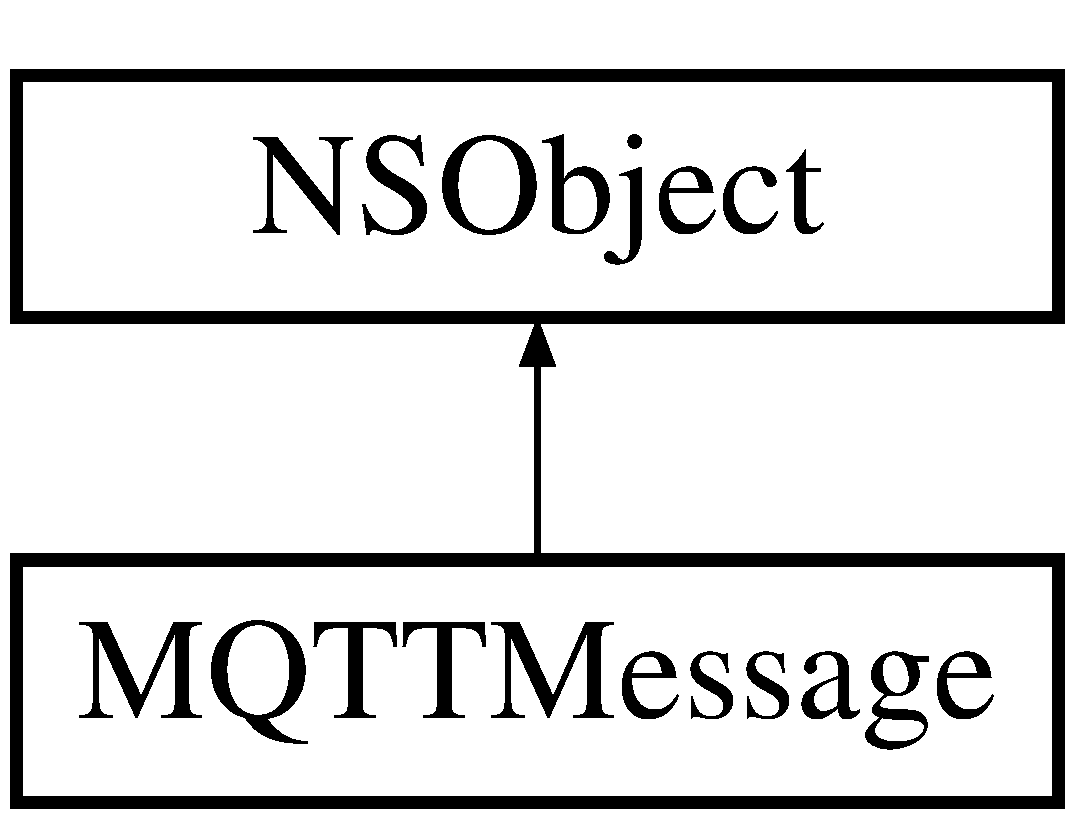
\includegraphics[height=2.000000cm]{interface_m_q_t_t_message}
\end{center}
\end{figure}
\subsection*{Instance Methods}
\begin{DoxyCompactItemize}
\item 
(id) -\/ \hyperlink{interface_m_q_t_t_message_a3a89c41b3fcd39e832f25c0e6e9729d0}{init}
\end{DoxyCompactItemize}
\subsection*{Properties}
\begin{DoxyCompactItemize}
\item 
unsigned short \hyperlink{interface_m_q_t_t_message_ae832d3bd3348f97c4a5bf86fd8e0c726}{mid}
\item 
N\-S\-String $\ast$ \hyperlink{interface_m_q_t_t_message_aea41fbd478102a49878498376a273705}{topic}
\item 
N\-S\-String $\ast$ \hyperlink{interface_m_q_t_t_message_ac2974959b4fca4589e4b6fc9f044f41e}{payload}
\item 
unsigned short \hyperlink{interface_m_q_t_t_message_af430192b287cfb6ef131f7e3d89249ef}{payloadlen}
\item 
unsigned short \hyperlink{interface_m_q_t_t_message_ae851052977c7286537111ec4072a1ab2}{qos}
\item 
B\-O\-O\-L \hyperlink{interface_m_q_t_t_message_aa7649c2ce6f7722f8038396744669389}{retained}
\end{DoxyCompactItemize}


\subsection{Method Documentation}
\hypertarget{interface_m_q_t_t_message_a3a89c41b3fcd39e832f25c0e6e9729d0}{\index{M\-Q\-T\-T\-Message@{M\-Q\-T\-T\-Message}!init@{init}}
\index{init@{init}!MQTTMessage@{M\-Q\-T\-T\-Message}}
\subsubsection[{init}]{\setlength{\rightskip}{0pt plus 5cm}-\/ (id) init 
\begin{DoxyParamCaption}
{}
\end{DoxyParamCaption}
}}\label{interface_m_q_t_t_message_a3a89c41b3fcd39e832f25c0e6e9729d0}
Initilizes new \hyperlink{interface_m_q_t_t_message}{M\-Q\-T\-T\-Message} \begin{DoxyReturn}{Returns}
a newly initialized \hyperlink{interface_m_q_t_t_message}{M\-Q\-T\-T\-Message} object 
\end{DoxyReturn}


\subsection{Property Documentation}
\hypertarget{interface_m_q_t_t_message_ae832d3bd3348f97c4a5bf86fd8e0c726}{\index{M\-Q\-T\-T\-Message@{M\-Q\-T\-T\-Message}!mid@{mid}}
\index{mid@{mid}!MQTTMessage@{M\-Q\-T\-T\-Message}}
\subsubsection[{mid}]{\setlength{\rightskip}{0pt plus 5cm}-\/ (unsigned short) mid\hspace{0.3cm}{\ttfamily [read]}, {\ttfamily [write]}, {\ttfamily [atomic]}, {\ttfamily [assign]}}}\label{interface_m_q_t_t_message_ae832d3bd3348f97c4a5bf86fd8e0c726}
Message Id \hypertarget{interface_m_q_t_t_message_ac2974959b4fca4589e4b6fc9f044f41e}{\index{M\-Q\-T\-T\-Message@{M\-Q\-T\-T\-Message}!payload@{payload}}
\index{payload@{payload}!MQTTMessage@{M\-Q\-T\-T\-Message}}
\subsubsection[{payload}]{\setlength{\rightskip}{0pt plus 5cm}-\/ (N\-S\-String $\ast$) payload\hspace{0.3cm}{\ttfamily [read]}, {\ttfamily [write]}, {\ttfamily [atomic]}, {\ttfamily [retain]}}}\label{interface_m_q_t_t_message_ac2974959b4fca4589e4b6fc9f044f41e}
String that represents the payload of the message \hypertarget{interface_m_q_t_t_message_af430192b287cfb6ef131f7e3d89249ef}{\index{M\-Q\-T\-T\-Message@{M\-Q\-T\-T\-Message}!payloadlen@{payloadlen}}
\index{payloadlen@{payloadlen}!MQTTMessage@{M\-Q\-T\-T\-Message}}
\subsubsection[{payloadlen}]{\setlength{\rightskip}{0pt plus 5cm}-\/ (unsigned short) payloadlen\hspace{0.3cm}{\ttfamily [read]}, {\ttfamily [write]}, {\ttfamily [atomic]}, {\ttfamily [assign]}}}\label{interface_m_q_t_t_message_af430192b287cfb6ef131f7e3d89249ef}
Length of the payload \hypertarget{interface_m_q_t_t_message_ae851052977c7286537111ec4072a1ab2}{\index{M\-Q\-T\-T\-Message@{M\-Q\-T\-T\-Message}!qos@{qos}}
\index{qos@{qos}!MQTTMessage@{M\-Q\-T\-T\-Message}}
\subsubsection[{qos}]{\setlength{\rightskip}{0pt plus 5cm}-\/ (unsigned short) qos\hspace{0.3cm}{\ttfamily [read]}, {\ttfamily [write]}, {\ttfamily [atomic]}, {\ttfamily [assign]}}}\label{interface_m_q_t_t_message_ae851052977c7286537111ec4072a1ab2}
Quality of service that the message was sent with \hypertarget{interface_m_q_t_t_message_aa7649c2ce6f7722f8038396744669389}{\index{M\-Q\-T\-T\-Message@{M\-Q\-T\-T\-Message}!retained@{retained}}
\index{retained@{retained}!MQTTMessage@{M\-Q\-T\-T\-Message}}
\subsubsection[{retained}]{\setlength{\rightskip}{0pt plus 5cm}-\/ (B\-O\-O\-L) retained\hspace{0.3cm}{\ttfamily [read]}, {\ttfamily [write]}, {\ttfamily [atomic]}, {\ttfamily [assign]}}}\label{interface_m_q_t_t_message_aa7649c2ce6f7722f8038396744669389}
Flag for whether or not the message will be retained \hypertarget{interface_m_q_t_t_message_aea41fbd478102a49878498376a273705}{\index{M\-Q\-T\-T\-Message@{M\-Q\-T\-T\-Message}!topic@{topic}}
\index{topic@{topic}!MQTTMessage@{M\-Q\-T\-T\-Message}}
\subsubsection[{topic}]{\setlength{\rightskip}{0pt plus 5cm}-\/ (N\-S\-String $\ast$) topic\hspace{0.3cm}{\ttfamily [read]}, {\ttfamily [write]}, {\ttfamily [atomic]}, {\ttfamily [retain]}}}\label{interface_m_q_t_t_message_aea41fbd478102a49878498376a273705}
String that represents the topic that the message was received on. 

The documentation for this class was generated from the following files\-:\begin{DoxyCompactItemize}
\item 
M\-Q\-T\-T\-Message.\-h\item 
M\-Q\-T\-T\-Message.\-m\end{DoxyCompactItemize}

%--- End generated contents ---

% Index
\newpage
\phantomsection
\addcontentsline{toc}{part}{Index}
\printindex

\end{document}
